\setcounter{chapter}{0}
\chapter{Meccanica Ondulatoria}
\section{La duale natura della materia}

\subsection{Esperimento della doppia fenditura}
Immaginiamo di condurre un esperimento in cui abbiamo uno spara palline posto difronte ad una parete e tra la parere e il macchinario \'e posto un separatore con due fenditure. Lo spara palline mantiene un certo rateo di fuoco e ruotando su un asse sparge le pallottole su un area angolare molto ampia. Ci aspettiamo che alcune di queste palline passino attraverso le fenditure, dunque posto un rilevatore sulla parete opposta al macchinario ed identificata una regione in cui le palline collidono contro il muro, possiamo domandarci quali sia la probabilit\`a che una pallina colpisca una certa area della superficie complessiva che possiamo indicare come $\Delta x$. Per rispondere a tale domanda costruiamo una distribuzione di probabilit\`a misurando le frequenza relative in un determinato arco di tempo rispetto all'area d'impatto. Ora ipotizziamo che le palline siano indistruttibili e che costituiscano un blocco indivisibile; ovvero se il ritmo con cui spara la macchina diminuisce di molto avremo che in ogni istante di tempo o il muro non viene colpito oppure arriva un solo proiettile. Inoltre la dimensione dei blocchi non dipendono dal rateo di fuoco della spara palline. Dunque possiamo dire che in ogni istante di tempo la dimensione dei blocchi \`e costante e questi sono distinti tra loro. Ripetendo l'esperimento costruiamo una distribuzione di probabilit\`a $P_{12}$ il cui valore \`e dato rispetto alla posizione lungo x. Tale probabilit\`a racchiude sia l'informazione che un proiettile possa passare dal foro 1 che dal foro 2.

 \begin{figure}[!ht]
\vspace{0.1in}
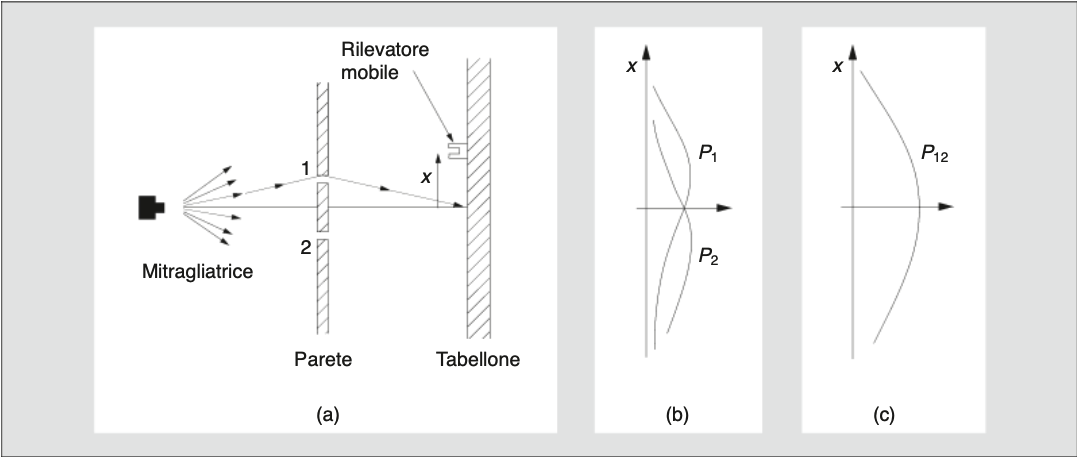
\includegraphics[width =11cm]{palla}	
\centering
\vspace{0.1in}
\caption{}
\end{figure}

\noindent Avremo che la probabilit\`a $P_{12}$ aumenta avvicinandosi a $x = 0$ e diminuisce al suo aumentare. Il fatto che la probabilit\`a sia massima nel centro \`e dovuto al fatto che se chiudiamo per esempio il foro 2 e costruiamo la distribuzione di probabilit\`{a} $P_1$ ripetendo l'esperimento, avremo che questa \`e massima nel punto in cui lo spara pallina mira nel centro della fenditura. Analogamente possiamo definire nello stesso modo chiudendo il foro 1 la probabilit\`{a} $P_2$. Confrontando le figure 1.1.b e 1.1.c si conclude che 
\begin{equation}
	P_{12} = P_1 + P_2
\end{equation}

\noindent Possiamo affermare che la probabilit\`a osservata con entrambe le fenditure \`{e} data dalla somma delle singole probabilit\`a quando una delle due \`e chiusa. Quando osserviamo una condizione di questo tipo diciamo che \textbf{non \`e presente interferenza}.

\subsubsection{Esperimento con Onde}

Ipotizziamo ora di fare lo stesso esperimento, ma anzich\`e utilizzare delle palline usiamo un contenitore d'acqua separato da una parete con due fenditure. A una delle due estremit\`a della scatola in posizione opposta al separatore \`e posto un motore che produce onde circolari. Per semplificare l'esperimento concettuale ipotizziamo che la parete della scatola, opposta la generatore di onde sia un perfetto assorbitore; solidarmente alla parete poniamo un rilevatore che misura l'intensit\`a del moto ondoso. \newline
Il rilevatore registra una grandezza che \`e proporzionale all'energia dell'onda o piuttosto all'energia che giunge al rilevatore.

\ 
\begin{figure}[!ht]
\vspace{0.1in}
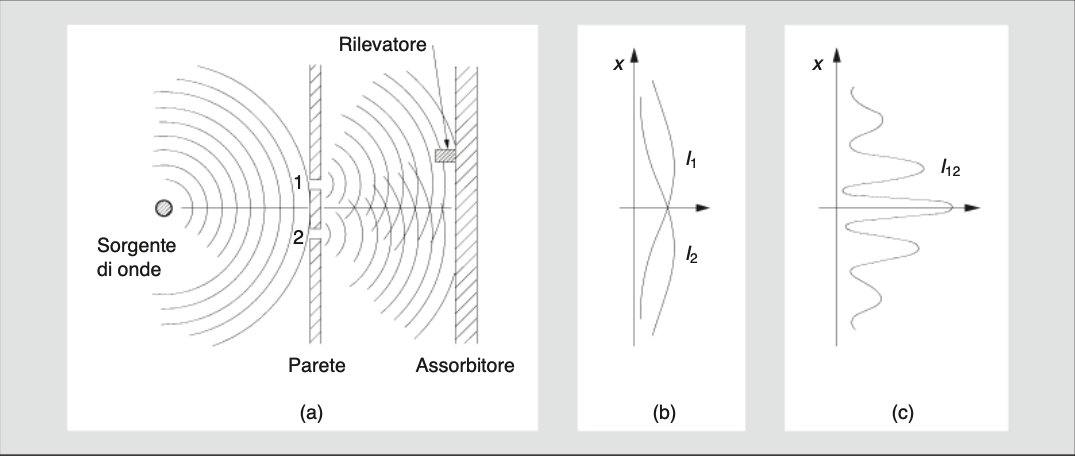
\includegraphics[width = 15cm]{onda}	
\centering
\vspace{0.1in}
\caption{}
\end{figure}

Misurando l'intensit\`a dell'onda per diversi valori di x (mantenedo costante il moto della sorgente delle onde), si ottiene una curva come quella in figura 1.2.c che identifichiamo come $I_{12}$. L'onda originale prodotta dalla sorgente, viene difratta attraverso i fori della parete di mezzo e dunque vengono generante nuove onde circolari con punto di diffusione coincidente con quello dei fori. Chiudendo un foro alla volta come fatto nell'esperimento delle palline si ottengono le singole distribuzioni d'intensit\`{a} rispetto a x date da $I_1$ e $I_2$ e rappresentante in figura 1.2.b. L'intensit\`{a} osservata quando i due fori sono aperti non coincide con la somma delle singole intensit\`a date da uno dei due fori chiusi. In questo caso diciamo che c'\`e \textbf{interferenza} tra le due onde. Dove la curva $I_{12}$ ha i suoi massimi diremo he le due onde sono in fase e i picchi delle onde si sommano, dando luogo a una grande intensit\`a. In tali punti l'interferenza \`e di tipo costruttivo tra le due onde. Un interferenza di questo tipo \`e possibile in tutti i punti dove la differenza delle distanza del rilevatore dai due fori \`e uguale ad un numero intero di lunghezze d'onda.

Nei punti in cui le onde arrivano al rilevatore con una differenza di fase di $\pi$, queste si dicono fuori fase e hanno un interferenza di tipo distruttivo, e l'intensit\`a dell'onda ne risulta diminuita. I valori pi\`u bassi in figura 1.2.c di $I_{12}$ avvengono in quei punti dove c'\`e interferenza distruttiva tra le onde. Si pu\`o dimostrare che i luoghi in cui $I_{12}$ \`e minima \`e nei punti in cui la distanza del rilevatore dal foro 1 differisce dalla distanza dal foro 2 di un numero dispari di lunghezze d'onda.

\noindent L'intensit\`a registrata dal rilevatore peer le onde provenienti da un singolo foro sono propozionali a
\begin{equation}
	I_i \simeq |h_i|^2 
\end{equation}
dove 
\begin{equation}
	h_i = h_ie^{i\omega t} 
\end{equation}
dove il termine $h_i \in \mathbb{C}$. L'intensit\`a rilevata a fenditure entrambe aperte sar\`a proporzionale a 
\begin{equation}
	I_{12} \simeq |h_1 + h_2|^2
\end{equation} 
sviluppando il termine si avr\`a che
\begin{equation}
	I_{12} \simeq |h_1|^2 + |h_2|^2 + 2Re(h_1\overline{h_2})
\end{equation}
L'equazione $I_{12}$ ci dice che $I_{12} \neq I_1 + I_2$ in quanto compare un termine aggiuntivo che descrive il fenomeno d'interferenza.

\subsection{Dualit\`a Onda - particella}

Quanto discusso nei punti precedenti anche se rappresentato da esperimenti concettuali descrive quella che \`e la duale natura della luce. Come sappiamo dalla fisica classica la luce \`e un onda elettromagnetica e come tale viene descritta dall'equazione dell'onda monocromatica
\begin{equation}
	\psi(x,t) = A e^{i(kx - \omega t)}
\end{equation}
e la sua intensit\`a \`e data da 
\begin{equation}
	I \simeq |\psi(x,t)|^2
\end{equation}
ma si comporta anche come una particella priva di massa, ovvero i fotoni. I medesimi risultati valgono anche nel caso di particelle con massa come gli elettroni. 


DESCRIVERE ESPERIMENTO CON ELETTRONI (AGGIUNGERE)

\subsection{La funzione d'onda}
La meccanica quantistica \`e una teoria probabilistica, ovvero si rinuncia all'assunzione della meccanica classica in cui l'evoluzione di un sistema \`e determinata a priori nel momento in cui si conoscono le leggi del moto e le condizioni iniziali di posizione e velocit\`a. Invece si assume che la natura del comportamento di un sistema sia del tutto probabilistica. La meccanica quantistica pu\`o determinare solo probabilisticamente la posizione di una particella nello spazio, ma non pu\`o asserirlo in modo deterministico come nel caso della meccanica classica. Infatti si ha una natura indetermistica dei risultati dovuta alla natura intrinsicamente probabilistica della teoria su cui la meccanica quantistica \`e costruita.

Per un onda di materia la densit\`a di probabilit\`a \`e associata all'intensit\`a con cui si misura l'energia trasportata dall'onda in un punto dello spazio in un tempo fissato $t_0$, ovvero
\begin{equation}
	P(x) = I(x) = |\psi(x,t_0)|^2
\end{equation}
Il termine a destra dell'equazione (1.8) prende il nome di \textbf{ampiezza di probabilit\`a}. Dalla densit\`a di probabilit\`a, \`e possibile calcolare la probabilit\`a effettiva moltiplicandola per il volume: la proobabilit\`a che una particella si trova in un volume infinitesimo dV con centro in un punto $\bold{x}$ \`e data da P($\bold{x},t)dV$.

Nel caso in cui consideriamo il volume esteso la probabilit\`a sar\`a espressa dall'integrale 
\begin{equation}
	P(\bold{x}) = \int_{V}|\psi(\bold{x},t)|^2dV
\end{equation} 
Poich\`e la funzione deve stare in un qualche posto \`e necessario che 
\begin{equation}
	\int_{V}|\psi(\bold{x},t)|^2dV = 1
\end{equation}
dunque la funzione d'onda $\psi(\bold{x},t)$ non pu\`o essere una funzione qualsiasi, ma deve appartenere all'insieme $L^2(\mathbb{R}^3)$ che \`e uno spazio di Hilbert. La condizione posta dall'equazione (1.10) ci dice che la probabilit\`{a} \`e \textbf{normalizzata}. Nel caso in cui si abbia una funzione d'onda per cui 
\begin{equation*}
	\int_{\mathbb{R}^3}dV|\psi(\bold{x},t)|^2 = N < +\infty
\end{equation*}
la funzione d'onda \`e normalizzabile costruendo una funzione d'onda 
\begin{equation*}
	\varphi(\bold{x},t) = \frac{1}{\sqrt{N}}\psi(\bold{x},t)
\end{equation*}
Notare che una funzione d'onda \`e normalizzabile solo se $\psi(\bold{x},t) \to 0 $ abbastanza rapidamente per $\bold{x} \to \infty$.

\noindent Una propriet\`a uitle delle funzioni d'onda \`e data dal risultato che se due funzioni differiscono tra loro per una costante, la fase complessa che li lega fa s\`i che descrivano lo stesso stato
\begin{equation*}
	\psi(\bold{x},t) = e^{i\alpha}\psi(\bold{x},t)
\end{equation*}

per una qualsiasi costante $\alpha \in \mathbb{R}$. In particolare la distribuzione di probabilit\`a rimane invariata. Combinando la condizione di normalizzazione e la non unicit\`a della fase, possiamo pensare agli stati di un sistema come un insieme quoziente formato da funzioni complesse normalizzabili che soddisfano la relazione di equivalenza 
\begin{equation}
	\varphi(\bold{x},t) \sim \psi(\bold{x},t) \iff \psi(\bold{x},t) = \lambda \psi(\bold{x},t) = \varphi(\bold{x},t)
\end{equation}
dove $\lambda \in \mathbb{C}$ e $\lambda \neq 0$. Dove le funzioni $\lambda \psi(\bold{x},t)$ e $\psi(\bold{x},t)$ descrivono lo stesso stato fisico.

\subsection{Principio di Sovrapposizione}
L'insieme delle funzioni d'onda dato da $L^2(\mathbb{R}^3)$ \`e uno spazio di Hilbert e dunque uno spazio vettoriale dotato di prodotto interno. Dunque dati due elementi $\psi_1(\bold{x},t),\psi_2(\bold{x},t) \in L^2(\mathbb{R}^3)$ che rappresenetano due stati del sistema deve esiste anche lo stato
\begin{equation}
	\psi_{3}(\bold{x},t) = \alpha \psi_{1}(\bold{x},t) + \beta \psi_2(\bold{x},t)
\end{equation}
per ogni $\alpha,\beta \in \mathbb{C}$. Tale propriet\`a prende il nome di \textbf{principio di sovrapposizione}. 

\noindent Il principio di sovrapposizione ha importanti conseguenze fisiche. Supponiamo che a un tempo $t_0$ si ha una particella localizzata in prossimit\`a di un punto $\bold{X}$. In accordo con quanto discusso fin'ora la sua posizione sar\`a descritta dalla funzione d'onda Gaussiana
\begin{equation*}
	\psi(\bold{x},t_0) = \frac{1}{\sqrt{N}}e^{-a(\bold{x}-\bold{X})^2}
\end{equation*}
Se applichiamo il principio di sovrapposizione (1.12) avremo che 
\begin{equation*}
	\psi(\bold{x},t_0) = \frac{1}{\sqrt{N'}}\left( e^{-a(\bold{x}-\bold{X}_1)^2}+e^{-a(\bold{x}-\bold{X}_2)^2}\right )
\end{equation*}

per due posizioni arbitrarie $\bold{X_1}$ e $\bold{X}_2$. L'interpertazione di tale equazione ci dice che in qualche modo la particella di si \`e divisa in due e si trova contemporaneamente nei dintorni di $\bold{X}_1$ e $\bold{X}_2$. Dato che una particella \`e indivisibile tale risultato \`e pi\`u interpretabile nel dire che percorre due cammini o pi\`u differenti tra loro simultaneamente.
\section{Particelle e Onde di Materia}

\subsection{Onde di Materia}

Nel 1923 De Broglie formula l'ipotesi che le particelle di materia, come i fotoni, possono avere l'aspetto delle onde. Tale ipotesi viene concepita dallo studio di come gli atomi emettono o assorbono energia (radiazione EM), osservando sperimentale che lo spettro atomico \`e discreto, ovvero \`e costituito da righe spaziate tra loro. Un atomo assorbe o emette fotoni solo a determinate frequenze. Tale risultato \`e facilmente interpretabile nel momento in cui si ipotizza che l'energia degli atomi \`e quantizzata, ovvero l'informazione viene ricevuta in pacchetti di energia che possono assumere solo valori discreti. L'assorbimento o emissione di fotoni fa s\`i che l'energia compia un salto da $E_i$ a $E_j $ tra i livelli di energia permessi. La conservazione dell'energia implica che la frequenza $\nu_{ij}$ di un fotone che genera un salto deve soddisfare la relazione 

\begin{equation}
	h \nu_{ij} = |E_i -E_j|
\end{equation} 
dove il termine "h" prende il nome di \textbf{costante di Planck}.

\noindent Per una particelle di materia di energia E e quantit\`a di moto \textbf{p}, un'onda che possiede una frequenza angolare $\nu = 2\pi \omega$ e un vettore d'onda \textbf{k} valgono le seguenti relazioni
\begin{equation}
\left \{ \begin{array}{l}
	E = h\nu = \hbar \omega \\
	\bold{p} = \hbar \bold{k}
\end{array} \right.
\end{equation}
e la lunghezza d'onda \`e data dall'equazione 

\begin{equation}
	\lambda = \frac{2\pi}{|\bold{k}|} = \frac{h}{|\bold{p}|}
\end{equation}

\subsection{L'equazione di Schr\"odinger}

La funzione d'onda $\psi(\bold{x},t)$ ci fornisce l'informazione sullo stato del sistema. Vogliamo ora capire come questo stato evolva nel tempo. Per studiarne il comportamento introduciamo l'equazione di Schr\"odinger 

\begin{equation}
	\boxed{i\hbar \frac{\partial \psi}{\partial t} = \hat{H} \psi}
\end{equation}
dove la constante $\hbar$ prende il nome di \textbf{costante di Planck ridotta}. Il suo valore \`e 
\begin{equation*}
	\hbar = 1.05 \times 10^{-34} Js
\end{equation*}
In meccanica quantistica l'unit\`a di energia che si utilizza \`e l'elettronvolt (eV), che \`e definito dall'energia cinetica che un elettrone assume quando accelerato da una differenza di potenziale di 1 Volt. Abbiamo che 1 eV $\approx 1,6 \times 10^{-19} J$ e dunque 
\begin{equation*}
	\hbar = 6,58 \times 10^{-16} eVs  
\end{equation*}

In meccanica quantistica l'equazione di Schr\"odinger assume il significato che $\bold{F} = m\bold{a}$ ha nella meccanica classica.
\subsubsection{La Hamiltoniana}

Il termine $\hat{H}$ prende il nome di Hamiltoniana e diverse sue scelte descrivono diversi sistemi fisici. Il cappuccio sulla H, sta ad indicare che nel contesto della meccanica quantistica viene inteso come un operatore che agisce sullo spazio delle funzioni $L^2(\mathbb{R}^3)$. Dato un potenziale $V(\bold{x})$ e assumendo che le particelle non si muovano a velocit\`a relativistiche nello spazio la Hamiltoniana assume la forma
\begin{equation}
	\hat{H} = -\frac{\hbar^2}{2m}\nabla^2 + V(\bold{x})
\end{equation}
che \`e un operatore differenziale. Ovvero prende in pasto una funzione $\psi(\bold{x},t)$ e restituisce un'altra funzione dopo averla differenziata utilizzando l'operatore $\nabla^2$.

\noindent Nel nostro caso la Hamiltonina del sistema coincide con l'energia totale del sistema, ovvero
\begin{equation*}
	H = \frac{\bold{p}^2}{2m} + V(\bold{x})
\end{equation*}
 L'equazione ottenuta in (1.17) \`e data dal fatto che possiamo pensare alla quantit\`a di moto come ad un operatore differenziale
 \begin{equation*}
 	 p \to -i\hbar\nabla 
 \end{equation*}

\subsection{Principio della decomposizione spettrale per una funzione d'onda}

Ipotizziamo di misurare di effettuare una misura al tempo $t_0$ allora la funzione d'onda $\psi(\bold{x},t_0)$ \`e soluzione dell'equazione (1.16) e vale 
\begin{equation*}
	\frac{\hbar^2}{2m}\nabla^2 \psi(\bold{x},t_0) = V(\bold{x})\psi(\bold{x},t_0)
\end{equation*}
essendo $\hat{H}$ un operatore differenziale auto-aggiunto definito sullo spazio di Hilbert $L^2(\mathbb{R}^3)$ possiamo applicare il teorema della decomposizione spettrale. Per un operatore di questo tipo si hanno un numero discreto ( e numerabile) di autovalori, il cui insieme corrisponde alla regione classica in cui il moto \`e limitato (nei punti in cui l'energia cinetica \`e minima si ha inversione), insieme ad uno spettro continuo che contiene tutti quegli autovalori in cui la regione del moto classico non \`e limitata. Di conseguenza la misura $\psi(\bold{x},t_0)$ pu\`o essere scritta come 
\begin{equation}
	\psi(\bold{x},t_0) = \sum_{a}c_{a}\psi_{a} + \int_{\sigma(a)}dE a(e)\varphi_a
\end{equation}
dove $\sigma(a)$ \`e l'insieme dello spetto continuo.

\noindent Nel caso in cui si ha solo uno spettro discreto si ha che per ogni $\psi(\bold{x},t)$, la probabilit\`a $P(a)$ di trovare un autovalore "a" per la misura al tempo $t_0$ \'e data dalla decomposizione di $\psi(\bold{x},t)$ in termini della funzione $\psi_{a}(\bold{x})$
\begin{equation}
	\psi(\bold{x},t_0) = \sum_{a}c_{a}\psi_{a}
\end{equation}
Inoltre per una misurazione $\psi(\bold{x},t_0)$ gli unici valori che pu\`o assumere devono appartenere all'insieme degli autovalori dello spettro discreto dell'operatore H.
Notare che la probabilit\`a deve essere normalizzata e dunque 
\begin{equation*}
	P(a) = \frac{|c_{a}|^2}{\sum_{a} |c_{a}|^2}
\end{equation*}

\newpage 

\subsection{Equazione di Schr\"odinger Indipendente dal Tempo}

L'equazione di Schdr\"odinger (1.16) \'e un equazione alle derivate parziali. Per risolverla consideriamo un asantz in cui la soluzione \'e esprimibile come due componenti di spazio e tempo separate tra loro.
\begin{equation}
	\psi(\bold{x},t) = e^{-\omega t}\psi(\bold{x})
\end{equation}
andando a sostituire nell'equazione (1.16), abbiamo che questa assume la forma 
\begin{equation}
	\hat{H}\psi(\bold{x}) = E\psi(\bold{x}) \quad \text{dove} \quad E = \hbar\omega  
\end{equation}
tale equazione prende il nome di \textit{equazione di Schr\"odinger indipendente dal tempo}. Nelle sezioni successive vedremo che tale equazione ammette autovalori o autostati E, solo per determinati valori. Tali grandezze verrano interpretate come i livelli di energia del sistema.

\noindent Soluzioni della forma (1.20) vengono definiti \textit{stati stazionari}. Come visto nel paragrafo precedente (principio di sovrapposizione) tali stati stazionari possono essere scritti come combinazione lineare di diversi stati stazionari e costituiscono una soluzione generale dell'equazione (1.21).

\subsection{Particella Libera}

Consideriamo una particella nello spazio, non soggetta a forze, allora avremo che il potenziale \`e 
\begin{equation*}
	V(\bold{x},t) = 0 
\end{equation*}
dunque l'equazione di Schr\"odinger pu\'o essere espressa come 
\begin{equation}
	-\frac{\hbar}{2m}\nabla^2 \psi(\bold{x},t) = i\hbar \frac{\partial \psi(\bold{x},t)}{\partial t}
\end{equation}
tale equazione differenziale \`e ha come soluzione la funzione 
\begin{equation}
	\psi(\bold{x},t) = Ae^{i(\bold{k}\cdot\bold{x} - \omega t)}
\end{equation}
 dove A \`e una costante, $\bold{k}$ il numero d'onda. Sostituendo nell'equazione (1.22) questa diventa 
 \begin{equation}
 	\frac{\hbar^2}{2m}\nabla^2 \psi(\bold{x}) = E\psi(\bold{x})
 \end{equation}
dove gli autostati sono delle forma 
\begin{equation*}
	E = \frac{\hbar^2 \bold{k}^2}{2m}
\end{equation*}
dove applicando la condizione di De Broglie si deve avere che 
\begin{equation}
	\omega = \frac{\hbar \bold{k}^2}{2m}
\end{equation}
che lega momento angolare e numero d'onda tra loro. La soluzione (1.23) rappresenta un'onda piana. Se calcoliamo la distribuzione di probabilit\`a associata avremo che 

\begin{equation*}
	P(\bold{x}) = |\psi(\bold{x},t)|^2 = |A|^2
\end{equation*}
e dato che A \`e una costante, si ha che dato un volume dV con centro in $\bold{x}$, la probabilit\`a di misurare la posizione della particella in tale volume \`e uguale in tutto lo spazio considerato.
\newline

\noindent Il principio di sovrapposizione ci dice che una soluzione generale dell'equazione (1.24) \`e combinazione lineare di funzioni d'onda piane che soddisfano la condizione (1.25). Tale soluzione \`e data dalla funzione 

\begin{equation}
	\psi(\bold{x},t) = \frac{1}{(2\pi)^{3 \backslash 2}} \int g(\bold{k})e^{i(\bold{k} \cdot \bold{x}-\omega t)}d^3k
\end{equation}
dove $g(\bold{k})$ pu\`o essere una funzione complessa, a patto che sia sufficientemente regolare affinch\`e la funzione integranda sia integrabile.

\noindent L'equazione (1.26) \`e interpretabile come un \textbf{pacchetto d'onda}, dove il contributo di ciascuna onda monocromatica e piana \`e pesato dalla funzione $g(\bold{k})$. Per t = 0 la funzione d'onda assume la forma 
\begin{equation}
	\psi(\bold{x},0) = \frac{1}{(2\pi)^{3 \backslash 2}} \int g(\bold{k})e^{i\bold{k} \cdot \bold{x}}d^3k
\end{equation}
Si dimostra che la funzione $g(\bold{k})$ non \`e altro che la trasformata di Fourier della funzione $\psi(\bold{x},t)$:
\begin{equation}
	g(\bold{k}) = \frac{1}{(2\pi)^{3 \backslash 2}} \int \psi(\bold{x},0)e^{-i \bold{k} \cdot \bold{x}}d^3x 
\end{equation}

\subsubsection{Significato fisico della funzione g(k)}

Utilizzando le equazioni di De Broglie abbiamo che $\bold{p} = \hbar \bold{k} $ dunque \`e possibile riscrivere la funzione (1.26) rispetto alla quantit\`a di moto come 
\begin{equation*}
	\psi(\bold{x},t) = \frac{1}{(2\pi)^{3 \backslash 2}} \int g(\bold{k})e^{\frac{i}{\hbar}(\bold{p} \cdot \bold{x} - Et)}d^3p
\end{equation*}
dove 
\begin{equation*}
	E = \frac{\bold{p}^2}{2m}
\end{equation*}
di conseguenza la funzione $g(\bold{k})$ diventa in funzione di $\bold{p}$ e si scrive come 
\begin{equation*}
	g(\bold{p}) = \frac{1}{(2\pi)^{3 \backslash 2}} \int \psi(\bold{x},0)e^{-\frac{i}{\hbar}\bold{p} \cdot \bold{x}}d^3x
\end{equation*}
il cui modulo quadrato  esprime la densit\`a di probabilit\`a di misurare un certo momento $\bold{p}$. 
\newline

\noindent Se la distribuzione di probabilit\`a \`e correttamente normalizzata avremo che 
\begin{equation*}
	\int |g(\bold{p})|^2d^3p = \int_{\mathbb{R}^3} | \psi(\bold{x},0)|^2d^3x = 1
\end{equation*}
per le propriet\`a della trasformata di Fourier.
\newpage 

\section{Pacchetti d'onda}
\subsection{Forma di un Pacchetto d'Onda ad un tempo fissato}

Consideriamo una particella libera che si muove in una sola dimensione, ovvero la sua posizione \`e data $x \in \mathbb{R}$. La forma del pacchetto d'onda \`e determinata dalla funzione $\psi(\bold{x},0)$, ovvero dalla misura che effettuiamo in un certo tempo $t=0$ fissato. Consideriamo che la funzione $|g(k)|$ abbia la forma di una distribuzione Gaussiana.

 
\begin{figure}[ht]
\vspace{0.1in}
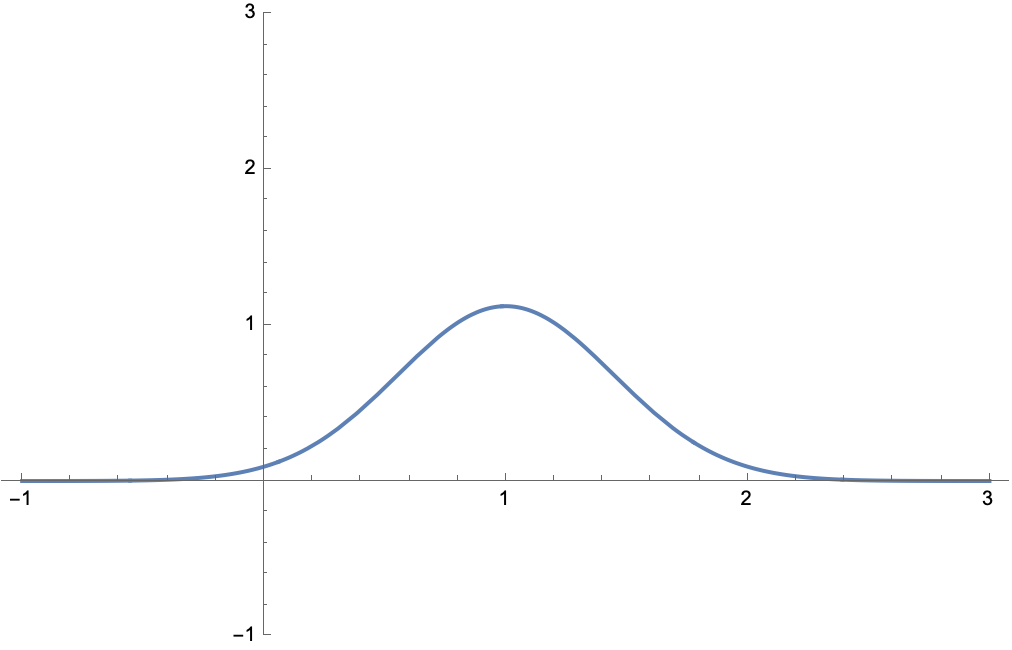
\includegraphics[width = 10cm]{gauss}	
\centering
\vspace{0.1in}
\caption{Grafico della funzione $g(k)$}
\end{figure}

\noindent dove g(k) ha un punto di massimo per $k = k_0$ che in figura 1.3 coincide con $k_0 = 1$ e inoltre la funzione ha ampiezza $\Delta k$ (che per esempio coincide con met\`a della sua ampiezza massima).
Per studiare il comportamento del pacchetto d'onda, consideriamo una caso particolare in cui
\begin{equation}
	\begin{aligned}
\psi(x) & =\frac{g\left(k_0\right)}{\sqrt{2 \pi}}\left[\mathrm{e}^{i k_0 x}+\frac{1}{2} \mathrm{e}^{i\left(k_0-\frac{\Delta k}{2}\right) x}+\frac{1}{2} \mathrm{e}^{i\left(k_0+\frac{\Delta k}{2}\right) x}\right] \\[0.5cm]
& =\frac{g\left(k_0\right)}{\sqrt{2 \pi}} \mathrm{e}^{i k_0 x}\left[1+\cos \left(\frac{\Delta k}{2} x\right)\right]
\end{aligned}
\end{equation}

ovvero la funzione d'onda $\psi(x,0)$ \`e sovrapposizione di un numero finto di funzioni d'onda con ampiezze $1, 1/2$ e $1/2$, dove la funzione d'onda \`e stata perturbata in un intorno di $k_0$. Osserviamo che la funzione (1.29) \`e massima per nel punto x=0, tale risultato \`e dato dal fatto che le onde in tale posizione formano un interferenza costruttiva. Spostandosi dal punto di massimo la funzione decresce fino a quando non raggiunge un punto di minimo dove l'interferenza distruttiva \'e massima; tale punto lo si raggiunge quando le onde hanno una differenza di fase di $\pm \pi$. Siccome la funzione (1.29) \`e una funzione continua, nel passaggio da massimo a minimo esiste sicuramente un punto sull'asse delle ascisse per cui la funzione si annulla, tale punto \'e dato da $x = \pm \frac{\Delta x}{2}$, dove 
\begin{equation}
	\Delta x \Delta k = 4 \pi
\end{equation}
L'equazione (1.30) ci dimostra che pi\`u piccola \`e l'ampiezza della funzione g(k) e maggiore \`e $\Delta x$ della funzione $\psi(x)$.
\newline

\noindent Consideriamo la funzione g(k) della forma \begin{equation*}
	g(k) = |g(k)|e^{i\alpha(k)}
\end{equation*}
assumiamo che $\alpha(k)$ ammetta derivata prima nell'intervallo $\left [k_0-\frac{\Delta k}{2}, k_0 + \frac{\Delta k}{2} \right ]$ allora possiamo sviluppare con Taylor in un intorno di di $k_0$ la funzione $\alpha(k)$

\begin{equation*}
	\alpha(k) \simeq \alpha(k_0) + \frac{d \alpha}{dk} \Big \vert_{k = k_0}(k-k_0)
\end{equation*}
sostituendo nell'equazione (1.27) in una sola dimensione si ha 

\begin{equation}
\psi(x, 0) \simeq \frac{\mathrm{e}^{i\left[k_0 x+\alpha\left(k_0\right)\right]}}{\sqrt{2 \pi}} \int_{-\infty}^{+\infty}|g(k)| \mathrm{e}^{i\left(k-k_0\right)\left(x-x_0\right)} \mathrm{d} k	
\end{equation}

dove il termine $x_0 = -\frac{d \alpha}{dk} \Big \vert_{k = k_0}$.
\newline

\noindent Quando $|x-x_0|$ \`e grande per x fissato, le fasi delle varie funzioni d'onda che formano $\psi(x,0)$ variano rapidamente nel dominio $\Delta k$, e tali onde ti distruggono a vicenda per il fenomeno d'interferenza. Se $x \simeq x_0$, la funzione integrata rispetto a k quasi non ha oscillazione e  $|\psi(x,0)|$ \`e massima.
La posizione $x_M(0) = x_0 $ coincide con il centro del pacchetto d'onda. L'integrale (1.27) assume valore massimo (in termini assoluti) quando le onde hanno l'ampiezza massima ($k \simeq k_0$) e hanno interferenza costruttiva. 
\newline
 
\begin{figure}[ht]
\vspace{0.1in}
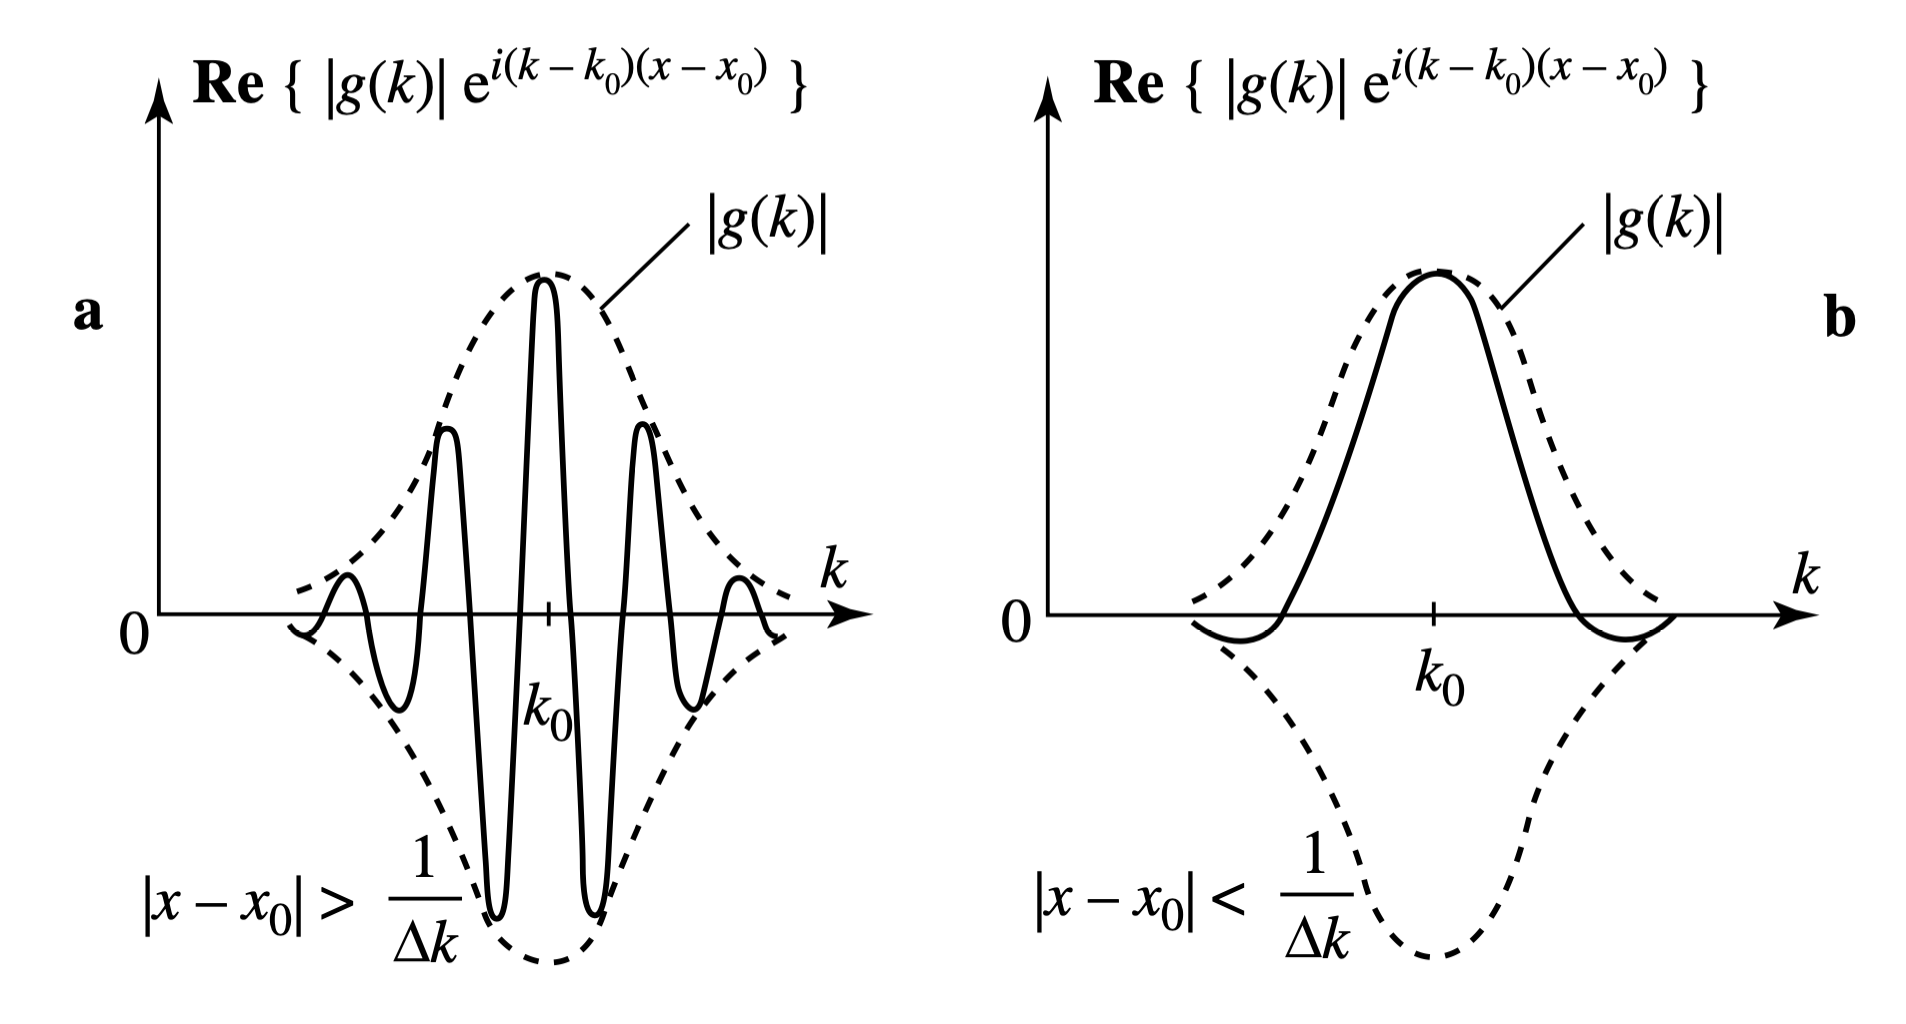
\includegraphics[width = 12cm]{packet}	
\centering
\vspace{0.1in}
\caption{}
\end{figure}

\noindent Quando x si allontana da $x_0$, la funzione $\psi(x,0)$ decresce. La diminuzione diventa significativa nel momento in cui $e^{i(k-k_0)(x-x_0)}$ compie almeno un oscillazione per k nel dominio $\Delta k$, questo accade quando

\begin{equation}
	\Delta k \Delta x \gtrsim 1
\end{equation} 

Tale risultato ci dice che il prodotto $\Delta k \Delta x$ ha un estremo inferiore; il cui valore preciso dipende dalla definizione di $\Delta x$ e $\Delta k$. Una pacchetto d'onda come quello dato dalla funzione (1.27) rappresenta una probabilit\`a, al tempo t=0, pressoch\`e nulla per  una posizione x, al di fuori dell'intervallo $\Delta x $ centrato su $x_0$.


\subsection{Principio d'Indeterminazione di Heisenberg}

Si \`e visto che per un'onda piana $e^{i(k_0x-\omega_0 t)}$ si ha che la densit\`a di probabilit\`a \`e costante in ogni punto dello spazio e in ogni tempo. Tale risultato pu\`o essere interpretato con il fatto che $\Delta x $ assume valore infinito e $\Delta k$ assume valore nullo. Per $k_0$ e $\omega_0$ fissati si ha che energia $E_0 = \hbar \omega_0$ e momento $p_0 = \hbar k_{0}$ sono ben definite. Per un onda piana di questo tipo, la definizione espressa in (1.27) pu\`o essere riscritta interpretando g(k) come una funzione delta
\begin{equation*}
g(k) = \delta(k-k_0) = 
\left \{\begin{array}{l}
	0 \quad k \neq k_0 \\
	+ \infty \quad k = k_0
\end{array} \right.
\end{equation*}
dunque possiamo esprimere la funzione (1.27) come 
\begin{equation*}
	\psi(x) = \frac{1}{\sqrt{2\pi\hbar }}\int \delta(k-k_0)e^{i\frac{p}{\hbar}x}dp = \frac{1}{\sqrt{2\pi \hbar}}
\end{equation*}
e dunque $|\psi(x)|^2 = \frac{1}{2 \pi \hbar}$ costante; di conseguenza la posizione \`e completamente indeterminata e la quantit\`a di moto \`e conosciuta con certezza assoluta.  
\newline

\noindent In termini probabilistici sappiamo che la probabilit\`a di misurare una certa quantit\`a di moto e una certa posizione sono definite dalle grandezze 
\begin{equation*}
	P(x) = \int_{- \infty}^{+\infty} |\psi(x,0)|^2dx \quad \text{e} \quad P(p) = \int_{-\infty}^{+\infty} |g(p)|^2dp
\end{equation*} 

dove le grandezze $\psi(x,0)$ e $g(p)$ sono legate tra loro dalla trasformazione di Fourier. Per tale legame vale il teorema di Plancherel
\begin{equation*}
	P(x) = \int_{- \infty}^{+\infty} |\psi(x,0)|^2dx  = \int_{-\infty}^{+\infty} |g(p)|^2dp
 =P(p)
\end{equation*}
di conseguenza ipotizzando che il valore degli integrali sia C, avremo che al tempo t = 0, misuriamo una probabilit\`a $dP(x) = \frac{1}{C}|\psi(x,0)|^2dx$ che la posizione della particella sia nell'intervallo $[x, x+ \Delta x]$ e nello stesso modo per la quantit\`a di moto che p sia nell'intervallo $[p,p + \Delta p]$.

\noindent Utilizzando le relazioni di De Broglie sappiamo che $\Delta p = \hbar \Delta k$, dunque possiamo riscrivere (1.32) come
\begin{equation}
	\Delta x \Delta p \gtrsim \hbar 
\end{equation}
\newpage 
\noindent Per una particella il cui stato \`e definito dal pacchetto d'onda (1.27), sappiamo che la probabilit\`a della sua posizione al tempo t=0 \`e definito solo in una regione $\Delta x$ con centro $x_0$; la sua posizione \`e conosciuta con una precisione $\Delta x$. Se si misura la quanti\`a di moto allo stesso tempo, il valore $p \in \left [p_0 - \frac{\Delta p}{2}, p_0 + \frac{\Delta p}{2} \right ]$, dato che $|g(p)|^2$ \`e nullo al di fuori di questo intervallo, la quantit\`a $\Delta p$ definisce la precisione con cui conosciamo p. 

\noindent La relazione (1.33) ci dice che fissato un istante di tempo \`e impossibile conoscere con precisione arbitraria la misura della posizione e quanti\`a di moto. Quando si raggiunge il limite inferiore dato da (1.33) aumentare la precisione con cui si conosce la posizione ($\Delta x$ diventa pi\`u piccolo) fa s\`i che la precisione con cui si conosce la quanti\`a di moto diminuisca ($\Delta p $ diventa grande); e viceversa. La relazione (1.33) prende il nome di \textbf{Principio d'indeterminazione di Heisenberg}.

\subsection{Evoluzione di un Pacchetto d'Onda}

Data un'onda piana $e^{i(kx-\omega t)}$ che propaga lungo l'asse Ox con velocit\`a di fase:

\begin{equation*}
	v_f(k) = \frac{\omega}{k}
\end{equation*}
Nel caso un onda elettromagnetica che si propaga nel vuoto la sua velocit\`a di fase \`e \`e costante d \`e data da $v_f = c $ dove c \`e la velocit\`a della luce. Per un onda di questo tipo tutte le onde che costituiscono il pacchetto d'onda si muovo alla stessa velocit\`a, e dunque il pacchetto si muove con la stessa velocit\`a, senza cambiare la sua forma. Nel caso in cui l'onda attraversi mezzi dispersivi, tale risultato non \`e pi\`u vero e la sua velocit\`a di fase \`e data da 
\begin{equation*}
	v_f(k) = \frac{\hbar k}{2m}
\end{equation*}
Tale equazione ci dice la velocit\`a con cui si propaga la singola onda del pacchetto, ma non la velocit\`a nel pacchetto nel suo complesso, per determinare tale grandezza consideriamo la funzione (1.26)

\begin{equation*}
	\psi(x,t) = \frac{1}{\sqrt{2\pi}} \int g(k) e^{i(kx-\omega(k)t)}dk
\end{equation*}

e consideriamo dei coefficienti della forma $g(k) = |g(k)|e^{-i \alpha(k)} $ e riscriviamo la funzione del pacchetto d'onda per un generico periodo t come 
\begin{equation*}
	\psi(x,t) = \frac{1}{\sqrt{2\pi}} \int dk|g(k)|e^{i(kx - \omega(k)t - \alpha(k))} 
\end{equation*}
Vogliamo determinare in quali regioni l'integrale ha un valore diverso da zero, ovvero non si ha interferenza distruttiva per $(x,y) \neq (0,0)$, e per farlo imponiamo la condizione per cui 

\begin{equation}
	\frac{d}{dk} \left [ kx - \omega t - \alpha \right] \approx  0
\end{equation}
risolvendo otteniamo che 
\begin{equation}
	x = \frac{d \omega}{dk}t + \frac{d\alpha}{dk}
\end{equation}
dove la grandezza
 
\begin{equation*}
	v_g = \frac{d \omega}{dk} 
\end{equation*}
prende il nome di \textbf{velocit\`a di gruppo} ed esprime la velocit\`a con cui si propaga il pacchetto d'onda.
Per un'onda di materia si ha che 
\begin{equation*}
	\omega  = \frac{E}{\hbar} = \frac{p^2}{2m \hbar } = \frac{\hbar k^2}{2m }
\end{equation*}
dunque la velocit\`a di gruppo del pacchetto \`e data da 
\begin{equation*}
	v_g = \frac{p}{m}
\end{equation*}

\subsubsection{Esempio - Evoluzione di un pacchetto Gaussiano}

Consideriamo la funzione d'onda rispetto ai momenti 

\begin{equation*}
	\psi(p) = g(p) = C e^{-\frac{\alpha(p-p_0)^2}{\hbar^2}} = Ce^{- \alpha k^2} = g(k)
\end{equation*}
La densit\`a di probabilit\`a dell'evoluto temporale della funzione sar\`a data da 
\begin{equation*}
|\psi(x,t)|^2 = \frac{C}{\sqrt{\frac{\alpha^2}{\hbar^2} + \frac{t^2}{4m^2}}} \exp{\left [ \frac{-\alpha}{4 \alpha^2 + \frac{\hbar^2 t^2}{m^2}}\left ( x - \frac{p_0}{m}t\right)^2\right]}
\end{equation*}
dove il centro del pacchetto d'onda si muove di moto rettilineo uniforme con
\begin{equation*}
	v_g = p_0/m
\end{equation*}
 e nel tempo la Gaussiana di allarga di un fattore 
 \begin{equation*}
 	\sigma(t) \sim \sqrt{4 \alpha^2 + \frac{\hbar^2 t^2}{m^2}}
 \end{equation*}
 
 \section{Comportamento Di un Pacchetto d'Onda In Presenza Di Un Potenziale }
 
 \subsection{Conservazione della probabilit\`a}
 
 Consideriamo una particella soggetta ad un potenziale che V(x,t) che dipende dal tempo, l'equazione di Schr\"odinger avr\`a la forma 
 \begin{equation}
 	i \hbar \frac{\partial \psi}{\partial t} = - \frac{\hbar}{2m} \nabla^2\psi +V(x,t)\psi 
 \end{equation}
tale equazione definisce l'evoluzione nel tempo di funzione d'onda. Le funzioni soluzione risultano essere normalizzate in modo tale che abbiano un interpretazione probabilistica. Vogliamo assicurarci che partendo da una funzione d'onda al tempo $t_0$ il suo evoluto ad un tempo $t > t_0$ ottenuto mediante la funzione (1.36) abbia ancora una descrizione probabilistica. Per dimostrare tale tesi, consideriamo l'evoluzione di $P(\bold{x},t) = |\psi(\bold{x},t)|^2  $ e studiamone l'evoluzione nel tempo
\begin{equation}
	\frac{\partial P}{\partial t}=\psi^{\star} \frac{\partial \psi}{\partial t}+\frac{\partial \psi^{\star}}{\partial t} \psi
\end{equation}
dove $\psi^*$ \`e il complesso coniugato della funzione $\psi$. Consideriamo l'equazione di Schr\"odinger e il suo complesso coniugato
\begin{equation*}
	\frac{\partial \psi}{\partial t}=-\frac{i}{\hbar}\left(-\frac{\hbar^2}{2 m} \nabla^2 \psi+V \psi\right) \quad \text { e} \quad \frac{\partial \psi^{\star}}{\partial t}=\frac{i}{\hbar}\left(-\frac{\hbar^2}{2 m} \nabla^2 \psi^{\star}+V \psi^{\star}\right)
\end{equation*}
 sostituendo nell'equazione (1.37)
 tali risultati si ha che l'evoluto temporale della densit\`a di probabilit\`a nel tempo \`e dato da 
 \begin{equation*}
 	\begin{aligned}
\frac{\partial P}{\partial t} & =\frac{i \hbar}{2 m}\left(\psi^{\star} \nabla^2 \psi-\psi \nabla^2 \psi^{\star}\right) \\[0.4cm]
& =\frac{i \hbar}{2 m} \nabla \cdot\left(\psi^{\star} \nabla \psi-\psi \nabla \psi^{\star}\right)
\end{aligned}
 \end{equation*}
 che riscriviamo nella forma 
 \begin{equation}
 	\frac{\partial P}{\partial t}+\nabla \cdot \mathbf{J}=0
 \end{equation}
 dove il termine $\bold{J}$ prende il nome di \textit{corrente di probabilit\`a} ed \`e dato da 
 \begin{equation}
 	\mathbf{J}=-\frac{i \hbar}{2 m}\left(\psi^{\star} \nabla \psi-\psi \nabla \psi^{\star}\right)ß
 \end{equation}
 Le equazioni della forma (1.38) sono conosciute come \textit{equazioni d continuit\`a} e compaiono quando sono presenti delle grandezze conservate.
 
 \noindent Si consideri un regione di spazio $\Omega \subseteq \mathbb{R}^3$ i cui contorno S. Determiniamo la probabilit\`a che una particella sia trovi in un  qualche punto nella regione $\Omega$ dello spazio, risolvendo l'integrale
 \begin{equation*}
 	P_\Omega(t) = \int_{\Omega} d^3x \; P(\bold{x},t)
 \end{equation*}
 L'equazione di continuit\`a ci dice che tale probabilit\`a cambia nel tempo come
 \begin{equation}
 	\frac{\partial P_\Omega}{\partial t}=-\int_\Omega d^3 x \; \nabla \cdot \mathbf{J}=-\int_S d \mathbf{S} \cdot \mathbf{J}
 \end{equation}
 dove nell'ultima equazione si \`e usato il teorema di divergenza. Dall'equazione (1.40) sappiamo che la probabilit\`a che la particella si trovi in un qualche punto della regione di spazio $\Omega$ cambia solo se \`e presente un flusso di probabilit\`a attraverso il suo contorno S. Se Sappiamo che $\bold{J} = 0$ ovunque sulla superficie S, allora la probabilit\`a che la particella sia nella regione $\Omega $ non cambia e dunque la probabilit\`a \`e costante nel tempo, ovvero
 \begin{equation*}
 	\frac{\partial P_{\Omega}}{\partial t} = 0
 \end{equation*} 
 
 \newpage
 
 \subsubsection{Particella in un potenziale indipendente dal tempo}
 
 Per un potenziale indipendente dal tempo si \`e visto nei paragrafi precedenti che l'equazione di Schr\"odinger (1.21) \`e indipendente dal tempo e che per una soluzione della forma (1.20) si hanno degli stati stazionari, ovvero degli stati dove l'energia del sistema \`e ben definita dato che $E = \hbar \omega$ ed $\omega$ \`e una valore fissato nel tempo per un'onda monocromatica. Essendo l'energia coincidente con la Hamiltoniana e dunque indipendente dal tempo si ha che in meccanica classica questa \`e una grandezza conservata, mentre in meccanica quantistica  si hanno stati di energia ben definiti. Data la forma della soluzione (1.20) la densit\`a di probabilit\`a \`e data da 
 \begin{equation*}
 	|\psi(\bold{x},t)|^2 = |\varphi(\bold{x})|^2
 \end{equation*}
 ovvero \`e indipendente dal tempo.
 
 \noindent Di conseguenza se consideriamo la l'equazione di continuit\`a in (1.38), sapendo che la densit\`a di probabilit\`a \`e indipendente dal tempo l'equazione diventa 
 \begin{equation*}
 	\nabla  \cdot \bold{J} = 0
 \end{equation*}
 dove per una dimensione si ha che 
 \begin{equation*}
 	\frac{\partial J_x}{\partial x} = 0
 \end{equation*}
 ovvero la corrente di probabilit\`a \`e costante.
 
 \subsubsection{Esempio}
 
 Nel caso di un'onda piana $\psi (x) = A e^{\frac{i}{\hbar}px}$ si ha che $|\psi(x)|^2 = |A|^2 $, ovvero la distribuzione di probabilit\`a \`e costante per posizione e tempo. La corrente di probabilit\`a \`e data da 
 \begin{equation*}
 	J = \frac{p}{m}|A|^2 = v|A|^2
 \end{equation*}
 tale risultalto \`e interpretabile come il flusso medio di particelle in una certa regione di spazio.
 
 \subsection{Regioni a potenziale costante}
 
 Consideriamo l'equazione di Schr\"odinger per un potenziale V(x) indipendente dal tempo e per semplicit\`a in una sola dimensione. L'equazione assume la forma 
 \begin{equation}
 	\frac{d}{d^2x}\varphi(x) + \frac{2m}{\hbar}(E-V)\varphi(x) = 0
 \end{equation}
Inoltre ipotizziamo che il potenziale sia costante $V(x) = V_0$ in alcune regione di spazio su cui \`e definito. Le soluzioni dell'equazione (1.41) cambiano in funzione di come cambia la grandezza E-V, dunque dobbiamo fare distinzione tra diverse casistiche:
\begin{enumerate}
	\item Per E  $ >V_0$ introduciamo la costante k data dalla relazione
	\begin{equation*}
		E-V_0 = \frac{\hbar^2 k^2}{2m}
	\end{equation*} 
	la soluzione per l'equazione (1.41) \`e della forma 
	\begin{equation*}
		\varphi(x) = Ae^{ikx}+A'e^{-ikx}
	\end{equation*}
	dove $A,A' \in \mathbb{C}$.
	\item Per $E < V_0$, si ha una condizione che corrisponde ad una regione di spazio che per una particella che segue le leggi della meccanica classica non sarebbe accessibile. In tal caso introduciamo la costante positiva $\rho$ definita da 
	\begin{equation*}
		V_0 - E = \frac{\hbar^2 \rho^2}{2m}
	\end{equation*}
	la soluzione per (1.41) \`e data da 
	\begin{equation*}
		\varphi(x) = Be^{\rho x} + B'e^{-\rho x}
	\end{equation*}
	dove $B,B' \in \mathbb{C}$.
	\item Per $E = V_0$ si ha che $\varphi(x)$ \`e una funzione lineare rispetto x.
\end{enumerate}

\subsubsection{Comportamento della funzione $\varphi(x)$  in punti in cui potenziale \`e discontinuo}

In casi in cui il potenziale \`e una funzione limitata, ma che possiede delle discontinuit\`a con salto, \`e necessario studiare il punto di singolarit\`a e determinare delle condizioni su come collegare i coefficienti delle varie regioni su cui si sono risolte le equazioni. In questi casi si impone che $\varphi(x)$ e $\varphi'(x)$ siano continue nel punto di discontinuit\`a e dunque le soluzioni debbano coincidere in tale punto.

\noindent Riscriviamo l'equazione (1.41) come 
\begin{equation}
	\varphi'' = \frac{2m}{\hbar^2}(V-E)\varphi
\end{equation}
Dato $x_0$ punto di discontinuit\`a per V(x), consideriamo un suo intorno $[x_0 - \varepsilon , x_0 + \varepsilon]$, ed integriamo (1.42) su tale intervallo.
\begin{equation*}
	\int_{x_0 - \varepsilon}^{x_0 + \varepsilon}dx \; \varphi'' = \frac{2m}{\hbar^2} \int_{x_0 - \varepsilon}^{x_0 + \varepsilon} dx \; (V-E)\varphi \; \to 0 \quad \text{per} \quad \varepsilon \to 0
\end{equation*}
tale equazione \`e equivalente ad imporre 
\begin{equation*}
	\varphi'(x_0+ \varepsilon) - \varphi'(x_0 - \varepsilon)  = \varphi'(x_0^+) - \varphi'(x_0^-) \to 0 \quad \text{per} \quad \varepsilon \to 0
\end{equation*}
di conseguenza $\varphi'(x_0)$ \`e continua e quindi anche $\varphi(x_0)$ \`e continua.
 
 \newpage
 
 \subsection{Potenziale a Gradino}
 
 Definiamo un potenziale  come una funzione a gradini
 \begin{equation*}
 	V(x) = \begin{cases}
 		0 \quad x < 0 \\
 		V_0 \quad x> 0 \\
 	\end{cases}	
 	\quad\quad\quad 
 	\vcenter{\hbox{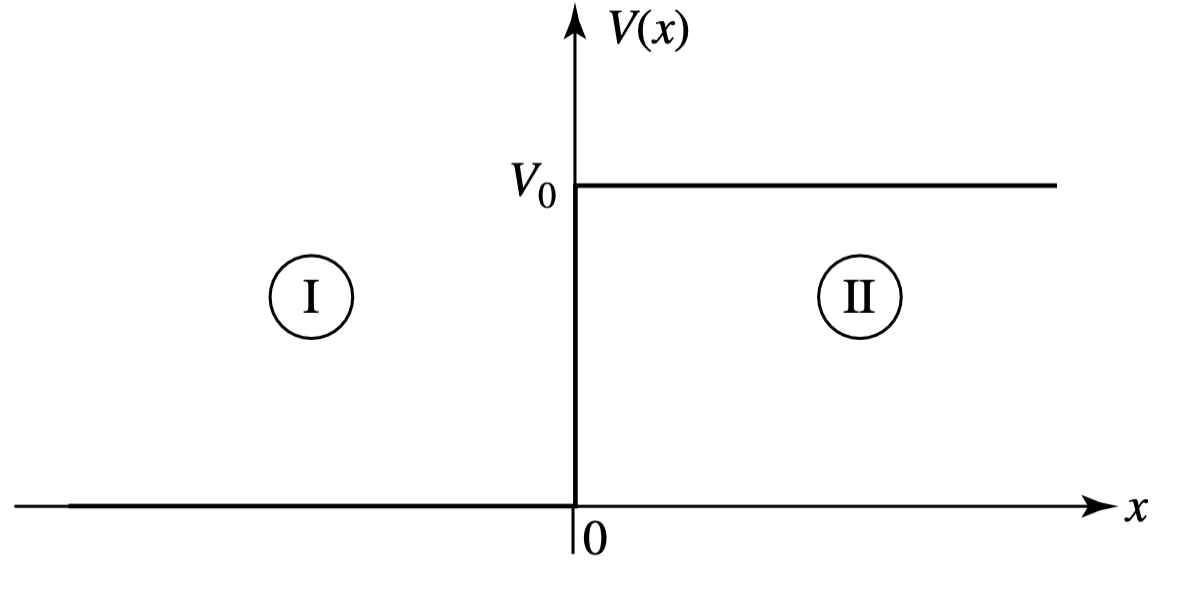
\includegraphics[width=8cm]{gradino}}}
 \end{equation*}
 Immaginiamo di sparare un fascio di particelle da sinistra e osservare che cosa succede. Quello che ci aspettiamo \`e che il fascio rimbalzi indietro se l'energia del fascio \`e minore del potenziale $V_0$, mentre se $E >> V_0$ non ci dovrebbero essere problemi nell'attraversare il gradino e la velocit\`a diminuisce. Per energie leggermente pi\`u grandi $V_0$, si hanno risultati interessanti.
\newline

\noindent  Per la regione (I) dove $x< 0$ consideriamo una soluzione di (1.41) della forma 
\begin{equation*}
	\psi_{1}(x) = Ae^{ik_1x}+A'e^{-ik_1x}
\end{equation*}
doe $k >0$ ed \`e dato da 
\begin{equation*}
	E = \frac{\hbar^2k_1^2}{2m}
\end{equation*}
tale soluzione include una parte della funzione d'onda che rimbalza contro il gradino e continua verso $x \to - \infty$, ma con momento opposto rispetto all'onda iniziale. L'onda entrante $e^{ikx}$ e quella di rimbalzo $e^{-ikx}$ hanno la stessa energia dato che risolvono l'equazione di Schr\"odinger per lo stesso stato, solo che la densit\`a di particelle del differisce, in generale ci aspettiamo che $A' < A$ e dunque parte dell'onda \`e stata assorbita e dunque non tutte le particelle del fascio tornano indietro.
\newline

\noindent Nella regione (II) dove $x > 0 $ e il potenziale vale $V(x) = V_0$, dato che il potenziale \`e costante la soluzione dell'equazione di Schr\"odinger associata \`e data da 
\begin{equation}
	\psi_2(x) = Be^{ik_2x}+B'e^{-ik_2x}
\end{equation}
dove il numero d'onda \`e dato da 
\begin{equation*}
	E-V_0 = \frac{\hbar^2k_2^2}{2m} \quad \Rightarrow \quad  k_2 = \sqrt{\frac{2m(E-V_0)}{\hbar^2}}
\end{equation*}
Si osserva che se l'energia del fascio di particelle \`e maggiore del salto del potenziale, $E > V_0$, il termine $k_2$ \`e reale. Se invece si ha che $E < V_0$, allora $k_2$ \`e un numero immaginario. 

\noindent Da un punto di vista fisico , per $E > V_0$ e dunque $k_2 \in \mathbb{R}$, interpretiamo la componente $Be^{ik_2x}$ della soluzione (1.43) come un onda che si propaga verso destra, mentre il secondo termine $B'e^{-ik_2x}$ \`e un onda che si propaga verso sinistra e che arriva $x \to + \infty$. Il problema \`e che il fascio i particelle arrivare da $x \to - \infty$ e dunque dobbiamo considerare solo soluzioni per cui $B' = 0$.

\noindent Si sarebbe giunti ad una conclusione uguale anche considerando un fascio di energia per cui $E < V_0$, in tal caso $k_2 = i\eta$ dove $\eta > 0$. In questo caso il secondo termine di (1.43) diventa $B'e^{-ik_2x} = B'e^{\eta x}$  che non \`e una funzione normalizzabile per $x \to + \infty$ e dunque soluzioni di questo tipo vengono scartate.
\newline

\noindent Dai risultati ottenuti nei punti precedenti possiamo concludere che la soluzione dell'equazione di Schr\"odinger \`e della forma
\begin{equation}
\psi(x) = \begin{cases}
	Ae^{ik_1x} +A'e^{-ik_1x} \quad x < 0 \\
	Be^{ik_2x} \quad x>0
\end{cases}	
\end{equation}
Per $x = 0 $ la funzione del potenziale V(x) ha un punto di discontinuit\`a con salto, nel paragrafo precedente abbiamo visto che le soluzioni date in (1.44) devono raccordarsi in tale punto e per farlo \`e necessario imporre delle condizioni al contro tali per cui $\psi(x)$ e $\psi'(x)$ siano funzioni continue.
\begin{equation}
	\left \{\begin{array}{l}
		\psi_1(0) = \psi_2(0) \\
		\psi_1'(0) = \psi_2'(0) 
	\end{array} \right.
	\iff
	\left \{ \begin{array}{l}
		A+B = C \\
		ik_1(A-B) = ik_2C
	\end{array}\right.
\end{equation}
Per le analogie della fisica ottica espresse dalle componenti delle soluzioni (1.44), identifichiamo con A la denesit\`a di particelle per il raggio di emissione iniziale, con B quella del raggio riflesso e con C quella del fascio trasmesso. 

\noindent Risolvendo il sistema (1.45) si ottengono i seguenti risultati
\begin{equation}
	B = \frac{k_1 - k_2}{k_1 + k_2}A \quad \text{e} \quad C = \frac{2k_1}{k_1 + k_2}A 
\end{equation}
Tali risultati possiamo interpretarli in termini di corrente di probabilit\`a o da un punto di vista fisico come flusso di particelle. Per il flusso originario si ha che 

\begin{equation*}
	J_{inc} = |A|^2\frac{\hbar k_1}{m}
\end{equation*}
La corrente del raggio riflesso \`e dato da
\begin{equation*}
	J_{rif} = |B|^2\frac{\hbar k_1}{m} = |A|^2\frac{\hbar k_1}{m} \left (\frac{k_1 - k_2}{k_1 + k_2}\right )^2 
\end{equation*}
dove per convenzione il flusso riflesso \`e considerato positivo. Infine il flusso trasmesso \`e 
\begin{equation*}
	J_{trasm} = |C|^2 \frac{\hbar k_2}{m} = |A|^2 \frac{\hbar k_2}{m}\frac{ 4k_1^2}{(k_1 + k_2)^2}
\end{equation*}
Ora ragioniamo su come interpretare questi risultati. Consideriamo il caso in cui $E > V_0$, in modo tale che $k_2 \in \mathbb{R}$. I questo caso le particelle riescono ad attraversare il gradino del potenziale. La domanda \`e come si comportano ? 
\newline

\noindent Per rispondere a tale domanda consideriamo il rapporto tra i flussi. Definiamo

\newpage

\begin{equation*}
	R = \frac{J_{rif}}{J_{inc}} = \left (\frac{k_1 - k_2}{k_1 + k_2} \right )^2
\end{equation*}

e
\begin{equation*}
	T = \frac{J_{trasm}}{J_{inc}} = \frac{4k_1k_2}{(k_1+k_2)^2}
\end{equation*}
tali rapporti prendono rispettivamente il nome di \textit{coefficiente di riflessione } e \textit{coefficiente di trasmissione}. Queste grandezze ci dicono quale frazione del flusso di particelle vengono riflesse e quali vengono trasmesse. In realt\`a dato che stiamo parlando di meccanica quantistica, quello che rappresentano \`e la probabilit\`a che una particella sia trasmessa o riflessa.
\newline

\noindent In particolare per tali coefficienti deve valere l'identit\`a 
\begin{equation*}
	R + T =1
\end{equation*}
che \`e definita per ogni potenziale e ci dice che nessun raggio di particelle viene disperso nell'interazione con il gradino di potenziale.

 
\begin{figure}[ht]
\vspace{0.1in}
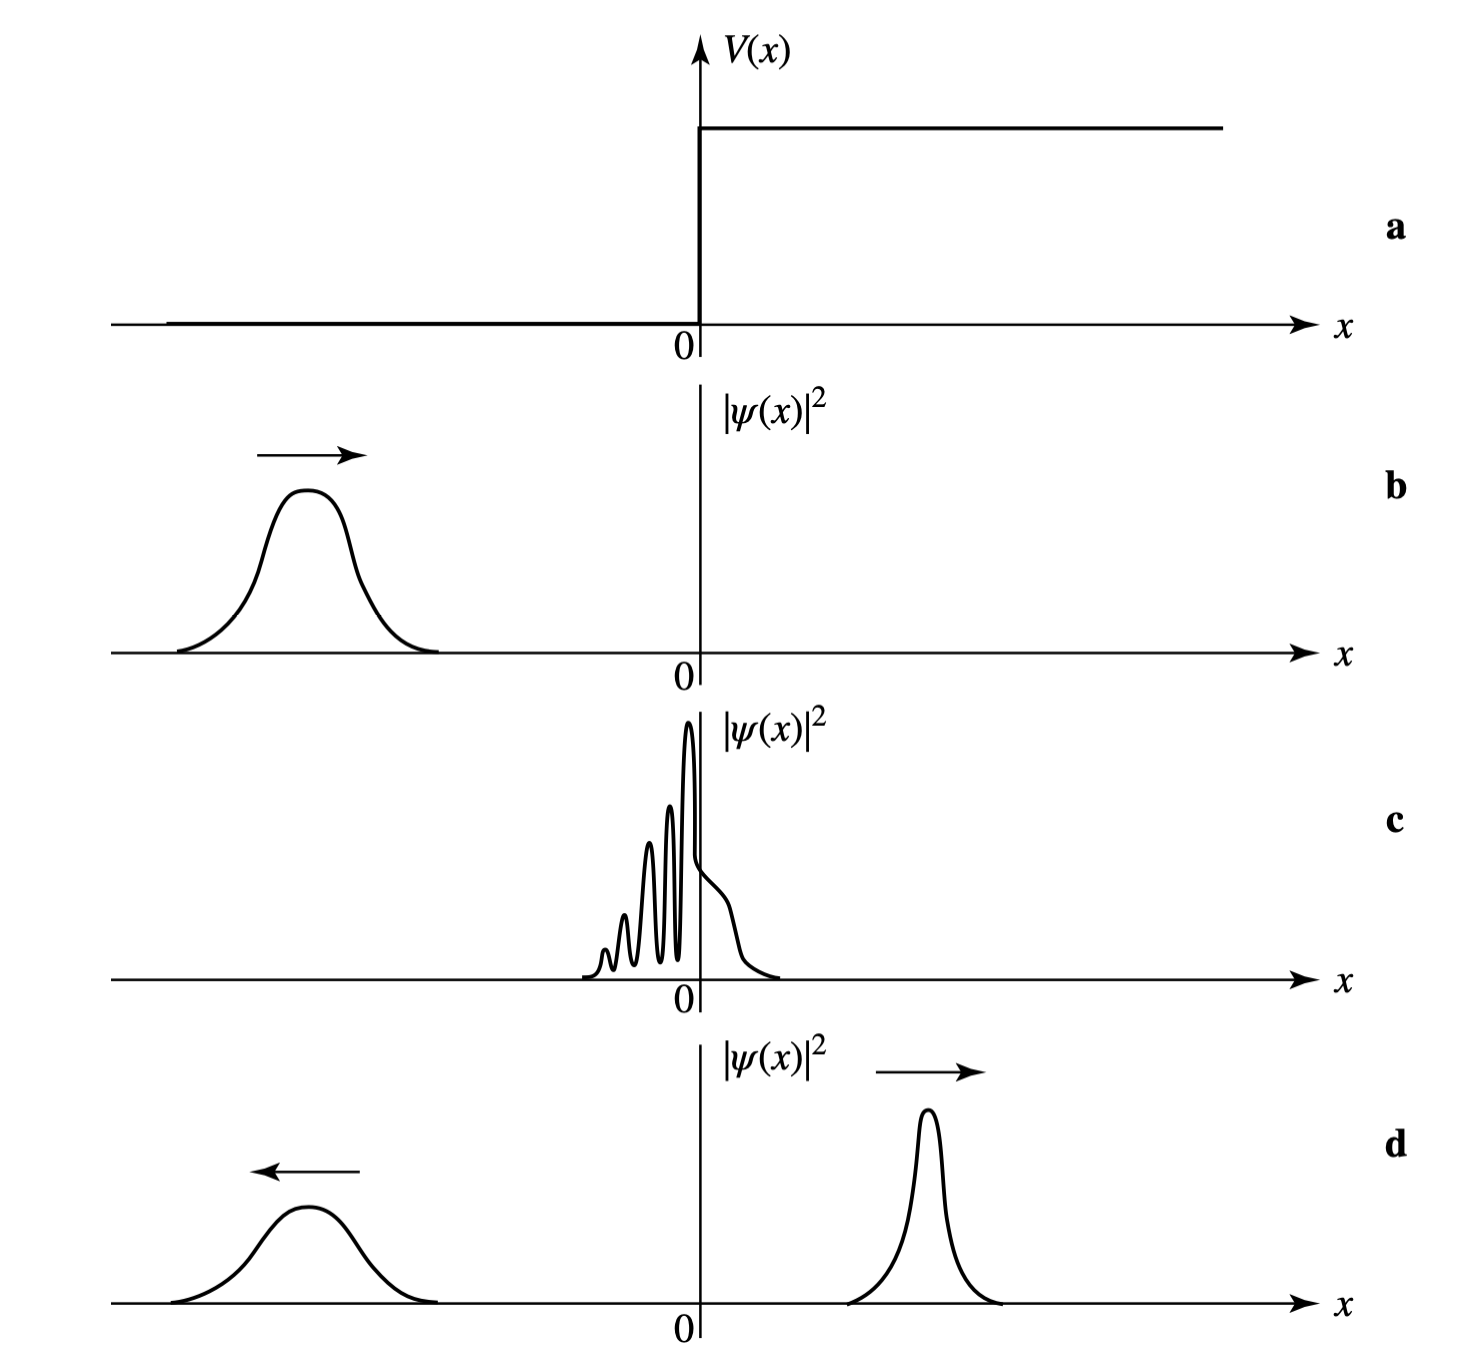
\includegraphics[width = 12cm]{reflect}	
\centering
\vspace{0.1in}
\caption{Si rappresenta il comportamento per un pacchetto d'onda che viene riflesso e trasmesso interagendo un potenziale a gradini per un energia $E > V_0$. Si osserva che il pacchetto riflesso ritorna con meno energia e una forma pi\`u schiacciata, ma con la stessa ampiezza del pacchetto originale. Mentre il pacchetto trasmesso ha una forma pi\`u piccata rispetto a quello di origine e una larghezza minore. Rispettivamente uno si propaga verso sinistra e l'altro verso destra.}
\end{figure}

\newpage

Resta da discutere il comportamento del raggio di particelle nel caso in cui $0< E < V_0$. In questo caso si ha che $k_2 \in \mathbb{C}$ e possiamo esprimerlo come $k_2 = i \eta$. Dunque la soluzione dell'equazione di Schr\"odinger per la regione del piano dove $x > 0$ diventa $\psi(x) = Be^{-\eta x}$, onde di questo tipo prendono il nome di onde evanescenti. Ripetendo quanto fatto per $E > V_0$ si ha che il coefficiente di trasmissione $T = 0$ e si ha $R=1$. Ovvero il fascio viene solo riflesso.
\newline

\noindent In realt\`a esistendo una soluzione reale nella regione del piano per $x > 0$ esiste una piccola probabilit\`a che il pacchetto d'onda possa attraversare un minimo la barriera per poi venire riflesso.

\subsection{Barriera di Potenziale (Effetto Tunnel)}
Dato il seguente potenziale limitato

 \begin{equation*}
 	V(x) = \begin{cases}
 		V_0 \quad 0< x < l \\
 		0 \quad \text{altrimenti} \\
 	\end{cases}	
 	\quad\quad\quad 
 	\vcenter{\hbox{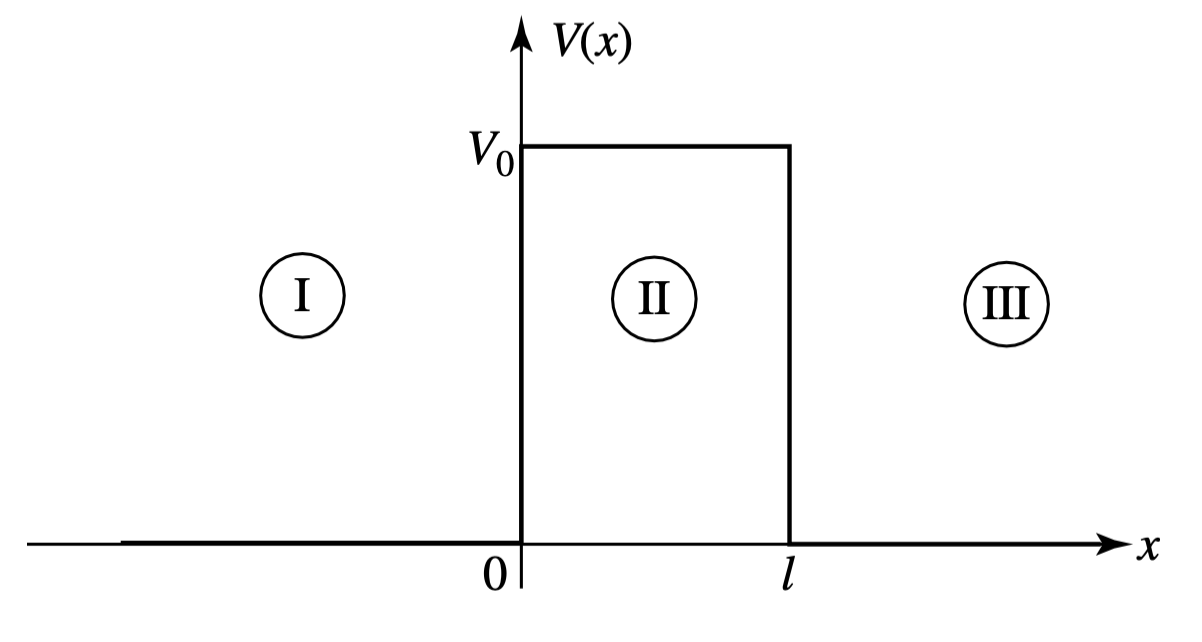
\includegraphics[width=8cm]{tunnel}}}
 \end{equation*}
 dove $V_0 > 0$. Il procedimento per risolvere l'equazione di Schr\"odinger \`e analogo a quello usato per il gradino del potenziale. L'unica differenza \`e che si ragione su 3 partizioni del piano e si determinato le soluzioni su di esse, per poi raccordarle nei punti di discontinuit\`a $x_1 = 0$ e $x_2 = l$ imponendo la condizione di continuit\`a per $\psi(x)$ e $\psi'(x)$. 
 
 \noindent Consideriamo l'energia per $E > V_0$, le soluzioni sono della forma 
 
 \begin{equation}
 	\psi(x) = \begin{cases}
 		A_1e^{ik_1x} + A_1'e^{-ik_1x} \quad x < 0\\
 		A_2e^{ik_2x} + A_2'e^{-ik_2x} \quad  0<x<l \\
 		A_3e^{ik_1x}
 	\end{cases}
 \end{equation}
 osserviamo che nella terza regione $k_1 = k_3$, dato che rispettivamente 
 \begin{equation*}
 	k_1 = k_3 = \sqrt{\frac{2mE}{\hbar^2}} \quad \text{e} \quad k_2 = \sqrt{\frac{2m(E-V_0)}{\hbar^2}}
 \end{equation*} 
 applicando le condizioni al contorno nei punti di discontinut\`a del potenziale, dopo alcuni passaggi algebrici otteniamo i coefficienti di riflessione e trasmissione 
 \begin{equation*}
 	R = \left |\frac{A_1'}{A_1} \right |^2 = \frac{(k_1^2 - k_2^2)sin^2(k_2l)}{4k_1^2k_2^2 + (k1^2-k_2^2)sin^2(k_2l)}
 \end{equation*}
 e
 \begin{equation*}
 	T = \left | \frac{A_3}{A_1} \right |^2 = \frac{4k_1^2k_2^2}{4k_1^2k_2^2 + (k1^2-k_2^2)sin^2(k_2l)}
 \end{equation*}
 \newpage 
 
 \noindent La probabilit\`a di riflessione oscilla al variare di $k_2$(ovvero dell'energia) e per $sin(k_2l) = 0 $ si ha T = 1.
 
 \noindent Nel caso in cui l'energia $0<E<V_0$ si ha che $k_2 = i\eta$ dove $\eta \in \mathbb{R}^+$ e dunque possiamo riscrivere il coefficiente di trasmissione come 
 \begin{equation*}
 	T = \frac{4k_1^2\eta^2}{4k_1^2\eta^2 + (k_1^2 + \eta^2)sinh^2(\eta l)}
 \end{equation*}
 Osserviamo che la probabilit\`a che la particella attraversi la barriera di potenziale non svanisce, tale risultato \`e in contrasto con la visione classica in cui il fascio di particelle dovrebbe essere solo riflesso. Tale fenomeno prende il nome di \textit{effetto tunnel}.
 \newline
 
 \noindent Per valori di $V_0 >> E$ o l molto grande si ha che $T \to 0$. L'effettp tunnel \`e importante per la descrizione dei fenomeni di decadimento radioattivo.
 
 \subsection{Buca di Potenziale dalle Pareti Infinitamente Grandi}
 
 Prendiamo in esame un potenziale della forma 
 \begin{equation*}
 	V(x) = \begin{cases}
 		0 \quad \text{altrimenti}\\
 		+ \infty \quad x \notin [0,a]
 	\end{cases} 
 	\quad \quad 
 	\vcenter{\hbox{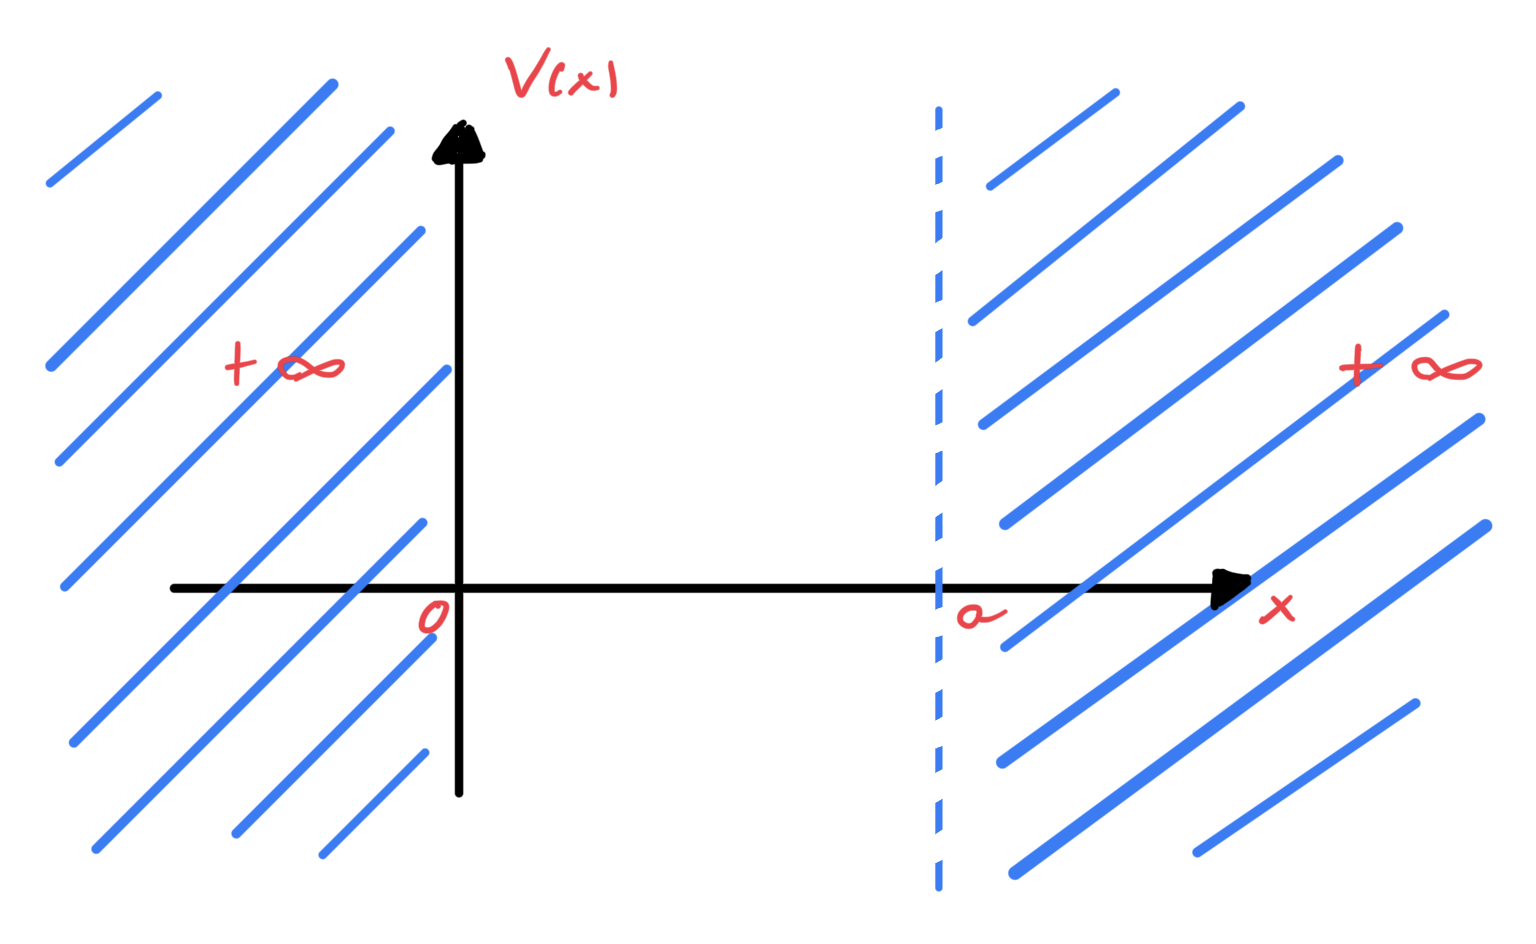
\includegraphics[width=9cm]{infinitewell}}}
 \end{equation*}
 e prendiamo in esame una particella trappola all'interno della buca di potenziale di larghezza "a" e pareti infinite. L'equazione di Schr\"odinger assume la forma 
 \begin{equation*}
 	-\frac{\hbar^2}{2m}\frac{\partial^2 \psi}{\partial x^2} + V(x)\psi = E \psi
 \end{equation*}
 Se vogliamo considerare solo stati di energia finiti, necessariamente avremo che per le regioni del piano in cui $V(x) = + \infty$ la funzione d'onda deve essere della forma $\psi(x) = 0$. Nella regione di spazio in cui il potenziale \`e nullo ritroviamo l'equazione che descrive l'evoluzione di una particella libera.
 \begin{equation}
 	-\frac{\hbar^2}{2m}\frac{\partial^2 \psi}{\partial x^2}  = E \psi
 \end{equation}
 Come fatto per la discussione dei potenziali precedenti dovremmo imporre la condizione che per $x = 0$ e $x = a$ la funzione d'onda $\psi(x) = 0$. Di conseguenza le funzioni d'onda saranno una restrizione della classe delle generiche funzione d'onda $e^{ikx}$. Consideriamo come ansatz di (1.48) la funzione 
 \newpage
 
 \begin{equation*}
 	\psi(x) = Ae^{ikx} + Be^{-ikx}
 \end{equation*}
con $k >0$. Imponendo la condizione $\psi(0) = 0$ sul bordo della buca del potenziale otteniamo le condizioni $B = -A$, dunque l'equazione precedente assume la forma 
\begin{equation*}
	\psi(x) = A(e^{ikx}-e^{-ikx}) = 2iA\sin(kx)
\end{equation*}
Il termine $2iA$ \`e una costante di normalizzazione e non influisce sulla descrizione della fisica del sistema. Imponendo la seconda condizione in cui $\psi(a) = 0$,abbiamo che 
\begin{equation*}
	\sin(ka) = 0 \Rightarrow k = \frac{n\pi}{a} \quad \text{per} \quad n \in \mathbb{Z}^+
\end{equation*}
 Per normalizzare la funzione calcoliamo
 \begin{equation*}
 	\int_0^a |\psi(x)|^2 = 1 \Rightarrow \int_0^a dx \; \sin^2 \left (\frac{n \pi x}{a} \right) = \frac{a}{2} \Rightarrow A = \frac{-i}{2}\sqrt{\frac{2}{a}}
 \end{equation*}
 e dunque la soluzione normalizzata diventa 
 \begin{equation}
 	\psi_n(x) = \sqrt{\frac{2}{a}}\sin\left (\frac{n \pi x}{a} \right )
 \end{equation}
 sostituendo all'interno dell'equazione (1.48) si ha che l'energia \`e quantizzata, ovvero pu\`o assumere valori solo su uno spettro di stati discreto.
 \begin{equation}
 	E_n = \frac{\hbar^2k_n^2}{2m} = \frac{\hbar^2 (n \pi)^2}{2ma^2}
 \end{equation}
 Quando una particella \`e vincolata a muoversi in regioni di spazio limitate, i livelli di energia si quantizzano perch\`e si formano delle onde stazionarie.
 
\begin{figure}[ht]
\vspace{0.1in}
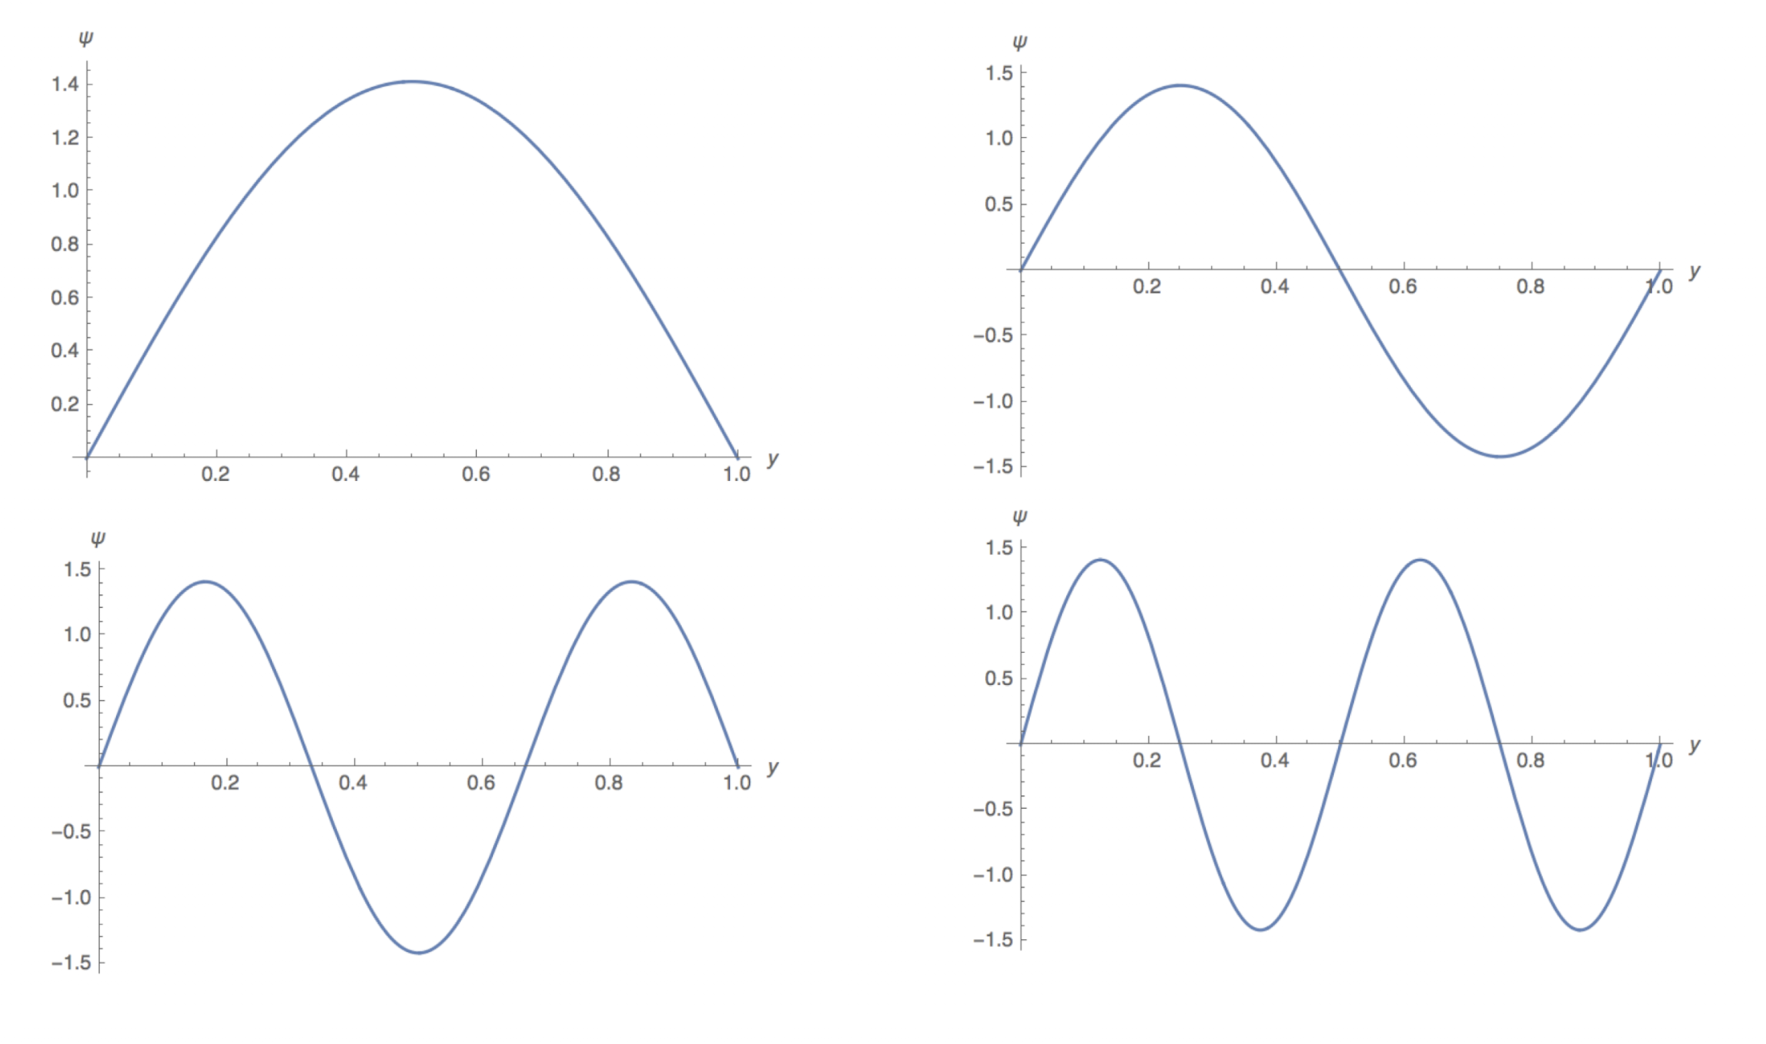
\includegraphics[width = 12.6cm]{groundstate}	
\centering
\vspace{0.1in}
\caption{funzioni d'onda stazionarie per n = 1,2,3,4.}
\end{figure}

\subsubsection{Propriet\`a di superposizione per gli stati stazionari}
Abbiamo che gli $E_n$ definiti dalla relazione (1.50) sono numeri reali e costituiscono gli autovalori dell'operatore Hamiltoniano H, di conseguenza le funzione d'onda $\psi_n(x)$ sono i corrispettivi autostati. Dunque $\{\psi_n(x)\}_{n \in \mathbb{N}}$ \`e una base ortonormale dello spazio $L^2([0,a])$, quindi una qualsiasi funzione $\psi(x)$ pu\`o essere scritta come combinazione lineare degli elementi della base 
\begin{equation}
	\psi(x) = \sum_{n=1}^{+ \infty}c_n \psi_n(x)
\end{equation}
dove i $c_n$ sono i coefficienti normalizzati. Essendo H un operatore lineare la funzione $\psi(x)$ espressa come nell'equazione (1.51) \`e soluzione dell'equazione di Schr\"odinger.
\newline

\noindent Come intuibile la particella rimane vincolata all'interno del pozzo, dunque possiamo pensare che le onde stazionarie che la rappresentano si muovano avanti e indietro all'interno delle pareti; di conseguenza la quantit\`a di moto non \`e ben definita in quanto $\psi(x) = e^{ikx} - e^{-ikx}$ e dunque \`e sovrapposizione di due stati che rappresentano rispettivamente due quantit\`a di moto distinte $p = \hbar k$ e l'altra $p = - \hbar k$.

\subsection{Buca di Potenziale Limitata}

Dato il potenziale 
\begin{equation*}
	V(x) = \begin{cases}
		-V_0 \quad x \in \left [-\frac{a}{2}, \frac{a}{2} \right ] \\
		0 \quad \text{altrimenti}
	\end{cases}
	\quad\quad\quad 
 	\vcenter{\hbox{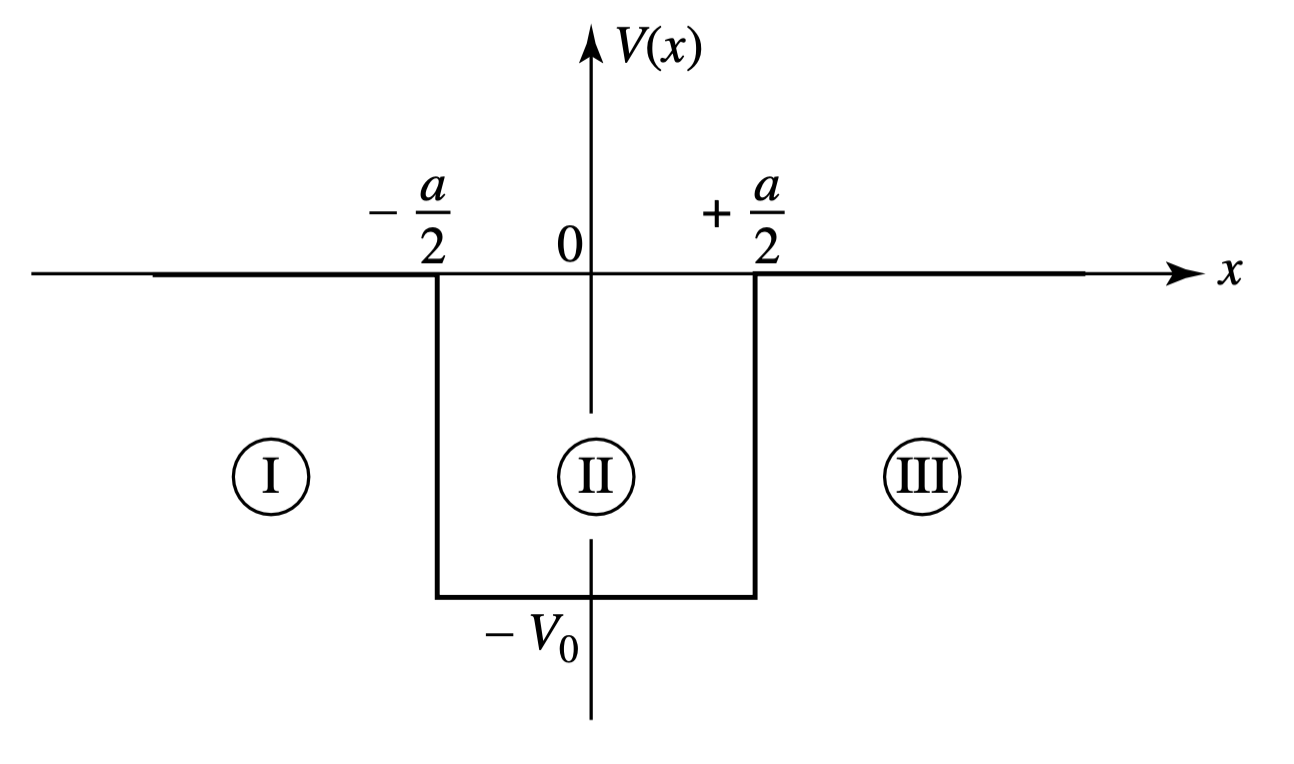
\includegraphics[width=8cm]{square}}}
\end{equation*}
dove $V_0 > 0$. Prima di proseguire con la ricerca della soluzione per l'equazione di Schr\"odinger associata, osserviamo che il potenziale \`e una funzione pari, ovvero V(-x) = V(x), questo vuol dire che tutte le soluzioni o sono funzioni pari o funzioni dispari. Osserviamo che se $\psi(x)$ \`e soluzione dell'equazione, allora anche $\psi(-x)$ deve esserlo, e dato che le soluzioni sono univoche e non possono esserci livelli di energia degeneri (ovvero un medesimo livello di energia associato a due funzioni distinte) dobbiamo avere che 
\begin{equation*}
	\psi(x) = \alpha \psi(-x)
\end{equation*}
per $\alpha \in \mathbb{C}$. Abbiamo che 
\begin{equation*}
	\psi(x) = \psi(-(-x)) = \alpha\psi(-x) = \alpha^2\psi(x)
\end{equation*}
dunque $\alpha = \pm 1$, di conseguenza la funzione pu\`o essere solo pari o dispari.

\subsubsection{Funzioni D'onda Pari}

Cerchiamo soluzioni per gli stati legati, per cui al di fuori del pozzo di potenziale abbiano la forma:
\begin{equation*}
\psi(x) = 
\begin{cases}
	Ae^{-i\eta x} \quad x > \frac{a}{2}\\
	Ae^{i\eta x} \quad x < -\frac{a}{2}
\end{cases}
\end{equation*}
dove $\eta \in \mathbb{R}^+$, scegliamo tali soluzioni in quanto vogliamo che la funzione d'onda sia una funzione $\psi \in L^2 \left (\left (-\infty,-\frac{a}{2} \right ] \cup \left [\frac{a}{2}.+ \infty \right )\right )$. Ci interessa sapere quali valori possa avere $\eta$ dato che questo determina l'energia degli stati legati, $E = -\frac{\hbar^2 \eta^2}{2m}$.
\newline 

\noindent All'interno dell'intervallo in cui il potenziale \`e non nullo, l'equazione di Schr\"odinger assume la forma
\begin{equation*}
	-\frac{\hbar^2}{2 m} \frac{d^2 \psi}{d x^2}=\left(E+V_0\right) \psi \quad -\frac{a}{2}<x< \frac{a}{2}
\end{equation*}
In base al valore dell'energia abbiamo due diversi tipi di soluzione 
\begin{itemize}
	\item Se $E < -V_0$ si hanno funzioni d'onda della forma $e^{\pm \rho x}$
	\item Se $E > -V_0$ si hanno funzioni d'onda della forma $e^{\pm ikx}$
\end{itemize}
Le soluzioni che ci interessano sono quelle per cui abbiamo gli stati legati e dunque ci limitiamo a studiare il comportamento del sistema per $-V_0 <E < 0$.

\noindent Dato che stiamo cercando soluzioni pari la funzione d'onda \`e data dalla combinazione lineare $\psi(x) = e^{ikx} + e^{-ikx}$ e dunque 
\begin{equation*}
	\psi(x) = B\cos(kx) \quad |x| < \frac{a}{2}
\end{equation*}
Non ci resta che applicare le condizioni al contorno per determinare le costanti di normalizzazione A e B. Dato che le funzioni dentro e fuori dalla buca sono pari \`e sufficiente applicare solo che condizioni per $\psi(-\frac{a}{2})$ e $\psi'(-\frac{a}{2})$, ottenendo
\begin{equation*}
\begin{cases}
	Ae^{-\eta \frac{a}{2}} = B \cos \left (\frac{a}{2}k \right ) \\
	kB \sin \left ( \frac{a}{2}k \right) = A\eta e^{-\eta \frac{a}{2}} 
\end{cases}
\end{equation*}
facendo il rapporto tra le funzioni abbiamo che 
\begin{equation*}
	\eta = k \tan \left (k \frac{a}{2} \right ) \iff \tan \left (k \frac{a}{2} \right ) = \frac{\eta}{k}
\end{equation*}
vogliamo determinare l'esistenza delle soluzioni al variare di k. Riscriviamo il termine di destra osservando che $k_0^2 = \frac{2mV_0}{\hbar^2}$ e dunque un generico stato k, possiamo scriverlo come $k^2 = k_0^2 - \eta^2$ e quindi
\begin{equation}
	\tan \left( \frac{a}{2}k \right ) = \sqrt{\frac{k_0^2 - k^2}{k^2}} = \sqrt{\left (\frac{k_0}{k} \right )^2 -1}
\end{equation}
essendo (1.52) un equazione trascendentale questa non ammette soluzioni esplicite, dunque si ricorre al metodo grafico per verificare l'esistenza di almeno una soluzione.

\newpage 
 
\begin{figure}[!ht]
\vspace{0.1in}
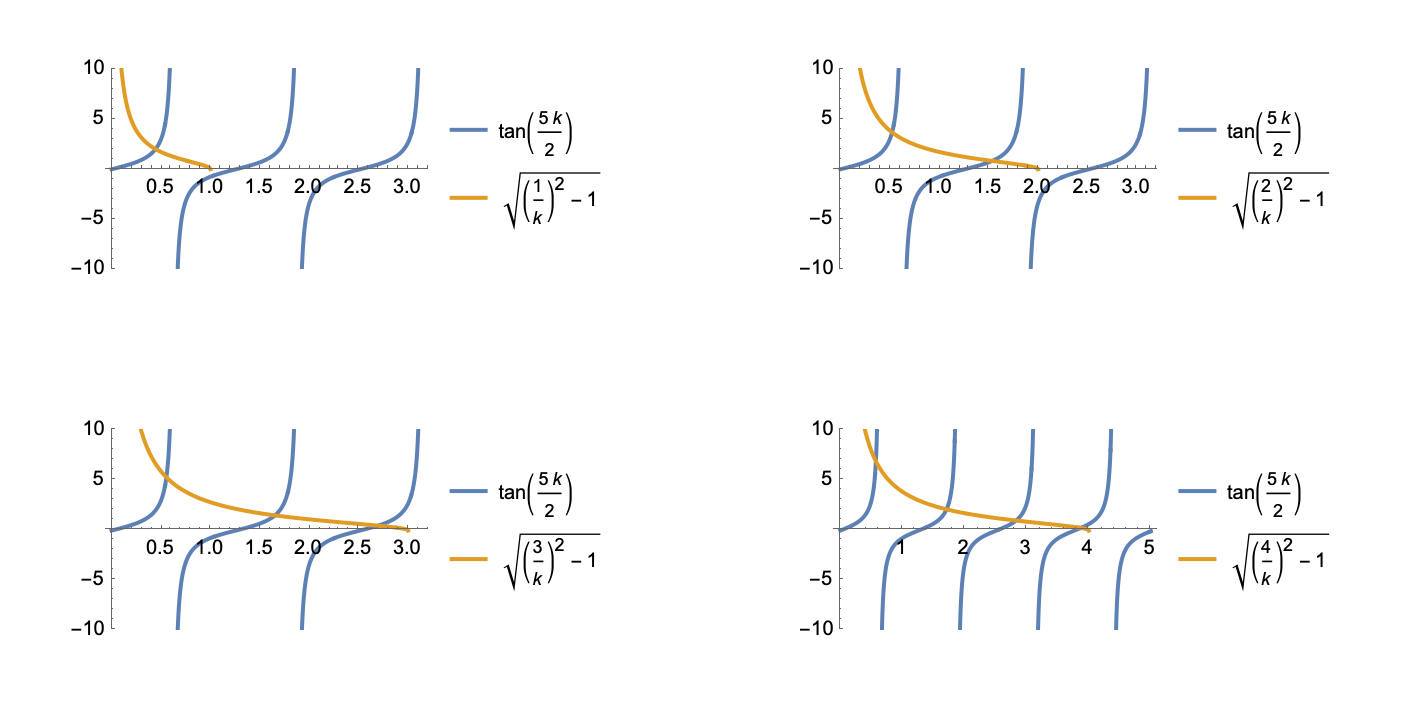
\includegraphics[width = 17cm]{k0}	
\centering
\vspace{0.1in}
\caption{Esistenza delle soluzioni al variare di $k_0 = 1,2,3,4$ e per una buca di ampiezza 5.}
\end{figure}
Come si osserva in figura 1.7 all'aumentare di $k_0$ e dunque del potenziale, il numero di soluzioni cresce. Per $V_0 \to + \infty$ si hanno un infinit\`a di soluzioni. Inoltre il numero di soluzioni dipende anche dalla costante "a" in quanto i punti in cui la tangente diverge ad infinito sono dati da $ k = \frac{n\pi}{a}$ per $n \in \mathbb{N}$. Infatti aumentando il valore di "a" abbiamo che le curve dipendenti da $k_0$ restano fisse, ma intersecano in pi\`u punti la funzione.
\newline

\noindent Il numero di stati legati \`e dato dalla relazione 
\begin{equation*}
	\frac{n\pi}{a} \leq k_0 \leq \frac{(n+1)\pi}{a}
\end{equation*} 
tale condizione \`e esprimibile rispetto al potenziale come
\begin{equation*}
	\frac{(n \pi)^2 \hbar^2 }{2ma^2} \leq V_0 \leq \frac{(n+1)^2 \pi^2 \hbar^2}{2ma^2}
\end{equation*}
Abbiamo visto che per livelli di energia $-V_0<E<0$ si hanno degli stati legati, e questo \`e quello che ci aspettiamo da un punto di vista classico per una particella confinata di una buca di potenziale. La parte interessante \`e che al di fuori della buca sono presenti delle funzioni d'onda decrescenti e questo vuol dire che per regioni che classicamente sarebbero inaccessibili si ha una probabilit\`a finita di trovare la particella al di fuori della buca.
\newpage 

\subsubsection{Funzioni d'onda dispari}
Analogamente a quanto fatto per le funzioni pari, al di fuori della buca di potenziale ricerchiamo delle funzioni della forma 
\begin{equation*}
\psi(x) = 
\begin{cases}
	Ae^{-\eta x} \quad x > \frac{a}{2}\\
	-Ae^{\eta x} \quad x < -\frac{a}{2}
\end{cases}
\end{equation*}
mentre all'interno della buca si ha una funzione della forma 
\begin{equation*}
	\psi(x) = B\sin(kx) \quad |a| < \frac{a}{2}
\end{equation*}
raccordando le soluzioni in $x = \frac{a}{2}$ si ottengono le condizioni al contorno
\begin{equation*}
	\begin{cases}
B \sin \left( k \frac{a}{2} \right ) = A e^{-\eta \frac{a}{2}} \\
k B \cos \left (k \frac{a}{2} \right)   =-\eta A e^{-\eta \frac{a}{2}}
\end{cases}
\end{equation*}
facendone il rapporto otteniamo
\begin{equation*}
	\cot \left (k \frac{a}{2} \right) = - \frac{\eta}{k} = - \sqrt{\left (\frac{k_0}{k}\right)^2 -1}
\end{equation*}
In questo caso non c'\'e garanzia dell'esistenza della soluzione. Essa esiste solo se il potenziale \`e profondo abbastanza o la buca larga a sufficienza.

\subsection{Potenziale a Funzione Delta}

Definiamo potenziale a funzione delta la seguente espressione
\begin{equation*}
	V(x) = -V_0\delta(x)
	\quad\quad\quad\quad\quad 
 	\vcenter{\hbox{\includegraphics[width=8cm]{delta}}}
\end{equation*}
dove $V_0 > 0 $. La funzione delta anche se definita in questo modo non \`e realmente una funzione, ma \`e una distribuzione che soddisfa le condizioni
\begin{equation*}
	\delta(x) = 
	\begin{cases}
		+ \infty \quad x  =  0\\
		0 \quad\quad\;  x \neq 0
	\end{cases}
	\quad \text{e} \quad \int_{-\infty}^{+\infty}dx\;\delta(x) =1
\end{equation*}
La discontinuit\`a data dalla funzione delta \`e molto pi\`u significativa di quella che si \`e vista per i potenziali con salto. Come fatto nei paragrafi precedenti per studiare il comportamento delle soluzioni in un intorno della discontinuit\`a integriamo la funzione di Schr\"odinger in un suo intorno.
\begin{equation*}
-\frac{\hbar^2}{2 m} \int_{-\epsilon}^{+\epsilon} d x \frac{d^2 \psi}{d x^2}=\int_{-\epsilon}^{+\epsilon} d x\left(E+V_0 \delta(x)\right) \psi
\end{equation*}
abbiamo che per $\varepsilon \to 0 $ l'equazione assume la forma 
\begin{equation}
	\lim_{\varepsilon \to 0} \left (\psi'(\epsilon) - \psi'(-\varepsilon) \right) = - \frac{2mV_0}{\hbar^2} \lim_{\varepsilon \to 0}\int_{-\varepsilon}^{+\varepsilon}dx \; \delta(x)\psi(x) = -\frac{2mV_0}{\hbar^2} \psi(0)
\end{equation}
dunque a differenza dei casi studiati nei precedenti paragrafi si ha una discontinuit\`a della derivata prima. La funzione d'onda comunque deve essere una funzione continua.
\newline

\noindent Consideriamo un livello di energia $V(x)<E<0$, rispettivamente avremo che la funzione d'onda per le due regioni di piano considerato deve assumere la forma 
\begin{equation}
	\psi(x) = \begin{cases}
		Ae^{-\eta x} \quad x < 0 \\
		Ae^{\eta x} \quad \;\; x > 0
	\end{cases}
\end{equation}
per $\eta >0$. Imponendo la condizione di continuit\`a della funzione d'onda abbiamo che 
\begin{equation*}
	\lim_{x \to 0^+} \psi(x) = \lim_{x \to 0^{-}}\psi(x) = A
\end{equation*}
e utilizzando la condizione di raccordo in (1.53) si ha che 
\begin{equation*}
\lim _{x \rightarrow 0^{+}} \psi^{\prime}(x)-\lim _{x \rightarrow 0^{-}} \psi^{\prime}(x)=-A \eta\left(\lim _{x \rightarrow 0^{+}} e^{-\eta x}+\lim _{x \rightarrow 0^{-}} e^{+\eta x}\right)=-2 A \eta
\end{equation*}
e quindi
\begin{equation*}
	\eta = \frac{mV_0}{\hbar^2}
\end{equation*}
In questo modo si \`e fissata l'energia del sistema trovando un solo stato legato possibile dato da
\begin{equation*}
	E=-\frac{\hbar^2 \eta^2}{2 m}=-\frac{V_0^2 m}{2 \hbar^2}
\end{equation*}
Tale risultato \`e caratteristico dei potenziali con funzione delta.
\newline

\noindent Consideriamo ora il livello di energia per $E > 0 $, in questo caso la soluzione dell'equazione di Schr\"odinger assume la forma 
\begin{equation}
	\psi(x) = \begin{cases}
 Ae^{ik_1 x} + Be^{-ik_1 x} \quad x < 0 \\
 C e^{ik_2x} \quad x>0	
 \end{cases}
\end{equation}
Il coefficiente A, rappresenta l'intensit\`a del fascio di particelle emesse in partenza, per comodit\`a consideriamo $A = 1$, inoltre $k_1 =k_2 = k$. Utilizzando le stesse condizioni discusse in precedenza si ha che 
\newpage

\begin{equation*}
	\begin{cases}
		1+B =C \\
		ikC - ik(1-B) = -\frac{2mV_0}{\hbar^2}C
	\end{cases}
\end{equation*}
svolgendo gli opportuni conti algebrici si trovano i corrispettivi valori della densit\`a di riflessione B e trasmissione C
\begin{equation*}
	\begin{cases}
		B = - \frac{mV_0}{mV_0 + ik\hbar^2} \\
		C = \frac{k\hbar^2}{mV_0 + ik \hbar^2}
	\end{cases}
\end{equation*}
Utilizzando tali risultati definiamo i coefficiente di riflessione e trasmissione
\begin{equation}
	R = |B|^2 = \frac{m^2V_0^2}{m^2V_0^2 + k^2\hbar^4} \quad \text{e} \quad  T = |C|^2 = \frac{k^2 \hbar^4}{m^2V_0^2 + k^2\hbar^4}
\end{equation}
Dallo studio delle soluzioni per $E < 0$ sappiamo che l'energia dello stato legato \`e data da 
\begin{equation*}
	E_L = -\frac{mV_0^2}{2\hbar^2} 
\end{equation*}
mentre l'energia della particella per $E>0$ \`e data 
\begin{equation*}
	E = \frac{\hbar^2k^2}{2m}
\end{equation*}
possiamo quindi pensare di riscrivere i coefficienti di trasmissione e riflessione in funzione dell'energia, nel seguente modo:
\begin{equation}
	T = \frac{E}{E + E_L} \quad \text{e} \quad R = \frac{E_L}{E+E_L}
\end{equation}
Un caso degenere \`e dato quando $E = - E_L$ dove i coefficienti tendono all'infinito. Fisicamente vuol dire che se prendiamo l'energia della particella che \`e positiva se la continuiamo analiticamente per valori negativi, avremo che l'ampiezza ha dei punti di polo per quei valori in cui si hanno gli stati legati. Dunque i coefficienti T ed R tengono conto dell'esistenza degli stati legati, mediante la loro relazione all'ampiezza di scattering.

\subsection{Comportamento di un Pacchetto d'Onda in un Potenziale a Gradini }

Consideriamo i risultati ottenuti nella sezione del potenziale a gradini a pagina \hyperlink{page.20}{20} e partendo dalla soluzione stazionaria (1.44), posto il coefficiente $A = 1$ consideriamo il suo evoluto temporale dato da:
\begin{equation}
\varphi(x,t) = 
\begin{cases}
	e^{i \left (k_1x - \frac{\hbar k_{1}^2}{2m}t \right)} + A'(k_1)e^{-i \left (k_1x + \frac{\hbar k_{1}^2}{2m}t \right)} \quad x<0 \\[0.5cm]
	C(k_1)e^{i \left (k_2x - \frac{\hbar k_{2}^2}{2m}t \right)} \quad x > 0
\end{cases}
\end{equation}
dove i numeri d'onda $k_1$ e $k_2$ sono legati dalla relazione
\begin{equation*}
	E_1 = E_2 \iff k_2^2 = k_1^2 - \frac{2mV_0}{\hbar^2}
\end{equation*}
Il risultato (1.58) definisce il comportamento per una sola onda, se vogliamo considerare un pacchetto d'onde dobbiamo applicare il principio di sovrapposizione e dunque definiamo 
\begin{equation}
	\psi(x,t) = \begin{cases}
		 \frac{1}{\sqrt{2 \pi}} \left [  \bigintsss dk_1 \; g(k_1)e^{i \left (k_1x - \frac{\hbar k_{1}^2}{2m}t \right)} + \bigintsss dk_1 \; g(k_1)A'(k_1)e^{-i \left (k_1x + \frac{\hbar k_{1}^2}{2m}t \right)}\right ] \quad x<0 \\[0.5cm]
	\frac{1}{\sqrt{2\pi}} \bigintsss dk_1 \;g(k_1)C(k_1)e^{i \left (k_2x - \frac{\hbar k_{2}^2}{2m}t \right)} \quad x > 0
	\end{cases}
\end{equation}

dove g(k) \`e una distribuzione il cui centro e media coincidono per un certo valore $k = k_0$. Per determinare come evolve il pacchetto d'onda nel tempo utilizziamo il metodo di fase stazionario dato dalla condizione (1.34) (pagina \hyperlink{page.15}{15}).  
\newline

\noindent Posto $g(k_1) = |g(k_1)|e^{-i\alpha(k_1)}$ i singoli termini del pacchetto d'onda assumono la generica forma 
\begin{equation*}
\int dk_1 \; |g(k_1)|F(k_1)e^{i(kx -Et - \alpha)}
\end{equation*}
Per determinare per quali valori di $k_1$ l'integrale \`e non nullo andiamo a cercare i punti in cui avviene interferenza costruttiva e dunque imponiamo la condizione
\begin{equation*}
	\frac{d}{dk_1} \left [ kx - Et - \alpha \right] = 0 \quad \iff \quad x-\frac{dE}{dk_1}t - \frac{d\alpha}{dk_1} \Big |_{k_1 = k_0} = 0
\end{equation*}
Per valori dell'energia $E > V_0$ e per $g(k)$ funzione reale. Abbiamo le condizioni sulle rispettive componenti sono date da: 
\begin{itemize}
	\item per l'onda incidente 
	\begin{equation*}
		x - \frac{\hbar k_0}{m}t \sim 0 \iff x_{inc} = \frac{p_0}{m}t
	\end{equation*}
	\item per l'onda riflessa 
	\begin{equation*}
		x + \frac{\hbar k_0}{m}t \sim 0 \iff x_{rif} = - \frac{p_0}{m}t 
	\end{equation*} 
	\item per l'onda trasmessa
	\begin{equation*}
		\frac{k_0x}{\sqrt{k_0^2 - \frac{2mV_0}{\hbar^2}}} - \frac{\hbar k_0}{2m}t \sim 0 \iff x_{tra} = \frac{p_2}{m}t
	\end{equation*}
\end{itemize}
dunque il pacchetto d'onda si muove con tre moti rettilinei diversi. Per tempi $t<0$ abbiamo che esiste solo il pacchetto d'onda incidente, dato che $x_{rif} > 0$ e l'onda riflessa in quella regione di piano non \`e definita, e analogamente $x_{tra} < 0$ e dunque non esiste. Se consideriamo $t > 0 $ avremo che esiste l'onda trasmessa $x_{trasm} > 0 $ e l'onda riflessa $x_{rifl} < 0$ che rispettivamente si propagano l'una in direzione opposta all'altra.
\newline
\noindent Se consideriamo livelli di energia in cui $0 < E < V_0$, abbiamo che nella seconda regione del piano il numero d'onda $k_2 = i \eta$ e dunque i termini di distribuzione di riflessione e trasmissione diventano termini complessi
\begin{equation*}
	A' = \frac{k_1 - i\eta}{k_1 +i \eta} \quad \text{e} \quad C = \frac{2k_1}{k_1 +i\eta}
\end{equation*}
osserviamo che il coefficiente di riflessione $R = |A'|^2 = 1$ di conseguenza dalla relazione $R + T = 1$ dobbiamo avere che $T = |C|^2 = 0$, se poniamo 
\begin{equation*}
	\eta^2 = \frac{2mV_0}{\hbar^2} - k_1^2 
\end{equation*}
sostituendo in C, abbiamo che 
\begin{equation}
	T = \frac{4k_1^2 \hbar^2}{2mV_0} = \frac{4E}{V_0} \approx 0 \iff E<<V_0 
\end{equation}
Procedendo analogamente a quanto fatto per il caso $E > V_0$, abbiamo che le condizioni per la parte di piano $x < 0 $ sono
\begin{equation*}
	\begin{cases}
		x_{inc} = \frac{p_0}{m}t \\
		x_{rifl} = -\frac{p_0}{m}t +\frac{d\alpha}{dk}|_{k=k_0}
	\end{cases}
\end{equation*}
dove il termine $\frac{d \alpha}{dk}|_{k=k_0}$ \`e un termine di sfasamento e dunque possiamo riscrivere il secondo termine come 
\begin{equation*}
	x_{rifl} = - \frac{p_0}{m}(t-\tau)
\end{equation*}
Da un punto di vista dinamico abbiamo che per $t<t_0$ \`e presente solo il pacchetto incidente, mentre per $t > t_0$ si ha solo il pacchetto riflesso. Ossserviamo che il coefficiente di trasmissione in (1.60) non \`e nullo di conseguenza esiste una probabilit\`a che le particelle si trovino nella regione del piano per $x > 0$, questo avviene per $t \approx \tau$, dove il pacchetto entra per un breve periodo nella regione inaccessibile. Pi\`u $E_0 = \frac{\hbar^2k_0^2}{2m}$ \`e vicino a $V_0$ e maggiore \`e il tempo $\tau$ di sfasamento. Il termine di sfasamento \`e dovuto al fatto che i coefficienti $A'$ e $C$ sono numeri complessi e dunque possiedono una fase.  